\documentclass[a4, 11pt]{article}

% #####################################################################################################################
\usepackage[utf8]{inputenc}
\usepackage[a4paper]{geometry}
\geometry{verbose,tmargin=4cm,bmargin=2.5cm,lmargin=2cm,rmargin=2cm,headheight=0.8cm,headsep=1cm,footskip=0.5cm}
\pagestyle{headings}
\setcounter{secnumdepth}{3}
\usepackage{url}
\usepackage{graphicx}
\usepackage{setspace}
% ############################################################################
% ############## Packages and Newcommands defined for AG #####################
% ############################################################################
\newcommand\hmmax{0}		% AG: odstraneni omezeni na pocet pouzitych fontu, obzvlast v AMS
\newcommand\bmmax{0}		% AG: odstraneni omezeni na pocet pouzitych fontu, obzvlast v AMS

\usepackage{amsfonts, amssymb, amsmath, amstext, amsthm}	        % math
\usepackage{physics}												% physics
\usepackage{braket}
\usepackage{esvect}                                                 % vectors with arrow, cmd is \vv{}
\usepackage{listings}		                                        % package for inserting codes
%\usepackage[framed,numbered,autolinebreaks,useliterate]{mcode}      % custom package in this dir, for m-code in latex
\usepackage{array, delarray}
\usepackage[utf8]{inputenc}                                         % english and also czech characters
\usepackage[czech]{babel}
\usepackage[IL2]{fontenc}                                           % zlepseni sazby v CZ. pripadne [T1], je to universalnejsi, nebo [IL2]
\usepackage{color, xcolor}                                          % defining package for some colors... also colors ("red", "green", etc.)
\usepackage{bm}
\usepackage{makeidx}                                                % makes index
\usepackage{hyperref}                                               % references
\usepackage{epstopdf, epsfig, graphicx}                             % pictures
\usepackage{blindtext, rotating}                                    % rotating images
\usepackage{epsfig}
\usepackage{float}                                                  % no floating figures in text anymore. Just add [H] behind begin figure!
\usepackage{booktabs, multirow}                                     % tables
\usepackage{hhline}
\usepackage{epigraph}                                               % citations
\usepackage{svg}		                                            % prime vkladani svg souboru

\usepackage{pdfpages}  												% prime vkladani pdf stranek pomoci prikazu \includepdf[pages=-]{myfile.pdf}
\usepackage{pgfplots}
%\usepackage{}
\usepackage[ddmmyyyy,hhmmss]{datetime}								% insert \today or \currenttime to see it
\usepackage{csquotes}
\usepackage{framed}

\usepackage{enumerate}
\usepackage[shortlabels]{enumitem}

\usepackage{shadethm}
\usepackage[stable]{footmisc}                                       % Load the footmisc package with the stable option

%\usepackage[scale=4.5, text=draft, color={[gray]{0.96}}]{draftwatermark}                                         % package for watermark 'draft' on each page


%\usepackage{watermark}                                         % package for watermarks  just add in document '\watermark{mytext}' and thats it.

%\usepackage[printwatermark]{xwatermark}

\usepackage{bm}


%%%%%%%%%%%%%%%%%%%%%%%%%%%%%%%%%%%%%%%%%%%%%%%%%%%%%%%%%%%%%%%%%%%%%
%% My unique commands in LaTeX
\newcommand{\ekviv}{ \Leftrightarrow }                           % ekvivalence (prave tehdy kdyz)
\newcommand{\commm}[1]{{\textcolor[cmyk]{0,1,0,0}{\textbf{\textsf{#1}}}}}      % new, commenting command, also red coloring
\newcommand{\com}[1]{\textbf{{\textsf{#1}}}}         % new, commenting command just comments
\newcommand\tab[1][1cm]{\hspace*{#1}}                % tabulator. tak jak ho zname z MS Wordu etc. 1cm
\newcommand{\slo}[1]{\medskip}                       % fakticky sloka pro verse
\newcommand{\uvoz}[1]{``{#1}''}                        % klasicke ENG uvozovky, vzdy funkcni... bylo drive {„{#1}“}

\newcommand{\chapquote}[3]{\begin{quotation} \textit{#1} \end{quotation} \begin{flushright} -- #2 \textit{#3}\end{flushright} }
% priklad na chapquote: \chapquote{Begin at the beginning,the King said gravely,and go on till you come to the end: then stop.}{Lewis Carroll}{Alice in Wonderland}
\renewcommand{\vec}[1]{\vv{#1}}  %{\boldsymbol{#1}}
\newcommand{\R}{ \ensuremath{\mathbb{R}} }

\newcommand{\setof}[1]{\ensuremath{\bm{\mathbf{#1}}}}				% mnozina prvku, vstup POUZE CAPSLOCK (funguje i na recka pismenka)
\newcommand{\alg}[1]{\ensuremath{\mathsf{#1}}}				% algebra 
\newcommand{\nv}[1]{\ensuremath{\mathcal{#1}}}			% nahodna velicina vstup POUZE CAPSLOCK
\newcommand{\deftxt}[1]{\textit{\textcolor{mygreen}{#1}}}			% nazev toho, co prave definuji (jen uvnitr definice)

\newcommand{\azar}{\ensuremath{  \land  }}			% symbol pro 'a zaroven'
\newcommand{\id}[1]{\ensuremath{  {}^I{#1}   }}				% velke I v predindexu, pro ideal v FPD

\newcommand{\oper}[1]{\ensuremath{\mbox{\textbf{\textsf{{\^{#1}}}}}}}				% operator (in QM or in general) ... bylo \mathsf{#1}
\newcommand{\mtx}[1]{\ensuremath{\mathbb{#1}}}

% Expectation symbol
\DeclareMathOperator*{\E}{\mathbb{E}}
% KLD operator
\DeclareMathOperator*{\KLD}{\mathrm{D}}

\renewcommand{\d}{\ensuremath{\mathrm{d}}}   % diferencial

\newcommand{\Hilsp}{ \ensuremath{\mathcal{H}}}   % Hilbert space

\newcommand{\dk}[1]{\begin{proof}#1\end{proof}}

\newcommand{\tequal}[1]{  \ensuremath{  \stackrel{\text{#1}}{=}  }  } % tequal{bla!} in math mode types equal sign with the specified text above it

% ######### helping to chop the words
\hyphenation{roz-ho-do-va-cích}
\hyphenation{Me-to-do-lo-gic-ky}
\hyphenation{for-ma-li-sa-tion}

% ######### defining my own colors
\definecolor{mygreen}{RGB}{3, 99, 50}   
\definecolor{myorange}{RGB}{3, 99, 50}

% ######### defining my math environmets
\theoremstyle{definition}
\newtheorem{definition}{Definition}{}


\newtheorem{temptheoforbackground}{Theorem}
\newenvironment{theorem}
{\colorlet{shadecolor}{green!15}
	\begin{shaded}  \vspace{-10pt}
		\begin{temptheoforbackground}
		}
		{
		\end{temptheoforbackground} \vspace{-10pt}
	\end{shaded}
}


\newtheorem{temppostulateforbackground}{Postulate}
\newenvironment{postulate}
{
	\colorlet{shadecolor}{orange!15}
	\begin{shaded} \vspace{-10pt}
		\begin{temppostulateforbackground}
		}
		{
		\end{temppostulateforbackground} \vspace{-10pt}
	\end{shaded}
}

\newtheorem{tempassumptionforbackground}{Assumption}
\newenvironment{assumption}
{
	\colorlet{shadecolor}{red!15}
	\begin{shaded} \vspace{-10pt}
		\begin{tempassumptionforbackground}
		}  
		{
		\end{tempassumptionforbackground} \vspace{-10pt}
	\end{shaded}
}



\theoremstyle{remark}
\newtheorem{remark}{Remark}{}

% ######### making index
\makeindex

%opening
\title{SKE protokol}

\author{Aleksej Gaj\footnote{email: \href{mailto:aleksejalex@gmail.com}{aleksejalex@gmail.com}}}

\begin{document}
	\maketitle	
	\tableofcontents
	
	\newpage
	
%	\begin{postulate}[Jen pro mně: censored vs died]
%		In the context of survival analysis, censored data refers to observations that are incomplete or not fully observed. Censoring occurs when the exact event time (such as death) for a subject is unknown or has not yet occurred at the end of the study or the time of analysis.
%		
%		In your dataset with patients, if the event of interest is whether they have died or not, the "censored" status indicates that the patient's event status is unknown because they were still alive or their follow-up time ended before the event occurred. It means that the patient was observed for a certain period but the event (death) did not occur within that period. Censoring can happen due to various reasons, such as the end of the study, loss to follow-up, or the patient being still alive at the time of analysis.
%		
%		In survival analysis, censored data is an important consideration. Statistical methods, like the Cox proportional hazards model or Kaplan-Meier estimator, handle censored data appropriately and use the available information to estimate survival probabilities and hazard rates.
%		
%		When analyzing your dataset, you would need to take into account both the "died" events and the censored observations to obtain valid estimates of survival probabilities or hazard ratios. The censored observations contribute information about the time the patient was followed until censoring, which is valuable in estimating the survival function beyond the observed events.
%		
%		It's crucial to appropriately handle and interpret censored data in survival analysis to obtain reliable conclusions about the survival experience of patients in your study.
%	\end{postulate}
%\newpage
	
	\section{Zadání}\label{sec:zadani}
	\textbf{A)} \textit{Pomocí parametrických a neparametrických metod pro cenzorovaná data odhadněte vhodný spolehlivostní model pro časy dožití (survt Tj) obou vybraných podskupin pacientů. Pro kontrolu fitu parametrické rodiny užijte Kaplan-Meierův plot nebo Nelson-Aalenův ‘hazard plot‘ (nejlépe v jednom obrázku spolu s parametrickým průběhem), resp. QQ/PP při RC.} \\
	\textbf{B)} \textit{SROVNEJTE tyto vybrané podskupiny vzhledem k jejich
	\begin{itemize}
		\item průběhu spolehlivosti (survival function) R(t), resp.
		\item intenzitě poruch (survivals) $ \lambda(t) $ (IFR/DFR/CFR), resp.
		\item kumulativní intenzitě poruch (survivals) $ \Lambda(t) $, resp.
		\item střední době života MTTF, resp.
		\item mediánové době života $ t_{med} $, resp.
		\item ...(jiné vlastní, pokud vás něco osloví)
	\end{itemize}} 
	\noindent
	\textbf{C)} \textit{Graficky srovnejte log-logR ploty pro obě podskupiny a na jejich základě zdůvodněte vhodnost/nevhodnost užití Coxova PH (proportional hazard) modelu.} \\
    
	\vfill{}
    
    \noindent
	\textbf{Skupina II.:}  treat=1(standard) versus treat=2(placebo) pro cell=2(small) \\
	
	\newpage
	
	\section{Dataset}\label{sec:dataset}
	Poskytnutý dataset představuje záznam testování vlivu jistého léčiva na dobu přežití pacienta. Data se skládají ze 137 pozorování 8 proměnných, viz Tabulka~\ref{tab:promenne_popis}. Cílem je modelovat dobu dožití (\textit{survival time}), tedy \texttt{survt} je vysvětlovaná proměnná.
	Ta je censorována podle proměnné \texttt{cens}. Další proměnné, které jsou k dispozici, představují věk pacienta, typ buněk, Karnofsky score (představující závažnost nemoci\footnote{Pozn: Hodnoty Karnofského skóre znamenají: $ KAR\leq30 $ -- úplná hospitalizace, $30<KAR\leq60$ -- částečná hospitalizace, $ KAR>60 $ -- vlastní péče bez hospitalizace.}), trvání nemoci (proměnná \texttt{didur}) a zda pacient už absolvoval léčbu v minulosti. 
	
	V této práci se zaměříme na skupinu pacientů s typem buněk \texttt{cell}=2. 
	
\begin{table}[H]
	\centering
	\begin{tabular}{@{}ll@{}}
		\toprule
		Název prom. & Komentář                    \\ 
		\midrule
		treat & treatment (1 = standard/lék, 2 = test/placebo)                    \\
		cell  & cell type (1 = squamous, 2 = small, 3 = adeno, 4 = large)         \\
		survt & survival time   (days)                                          \\
		cens  & status (0 = censored, 1 = died)                                 \\
		KAR   & performance status -- Karnofsky score (0 = worst,..., 100 = best) \\
		didur & disease duration from diagnosis to treatment (months)           \\
		age   & age (years)                                                     \\
		prith & prior therapy (0 = none, 10= some)                             \\
		\bottomrule
	\end{tabular}
	\caption{(Poskytnutý) popis proměnných v datasetu}
	\label{tab:promenne_popis}
\end{table}

V Tabulce~\ref{tab:zaklad_anal_cely_dataset} je uvedena základní analýza na celém datasetu, v Tabulce~\ref{tab:analyza_muj_dataset} pak analýza podskupiny \texttt{cell}=2.

\begin{table}[H]
	\centering
	\begin{tabular}{lrrrrrrrr}
		\toprule
		& treat & cell & survt & cens & KAR & didur & age & prith \\
		\midrule
		count & 137.00 & 137.00 & 137.00 & 137.00 & 137.00 & 137.00 & 137.00 & 137.00 \\
		mean & 1.50 & 2.34 & 121.63 & 0.74 & 58.57 & 8.77 & 58.31 & 2.92 \\
		std & 0.50 & 1.07 & 157.82 & 0.44 & 20.04 & 10.61 & 10.54 & 4.56 \\
		min & 1.00 & 1.00 & 1.00 & 0.00 & 10.00 & 1.00 & 34.00 & 0.00 \\
		25\% & 1.00 & 1.00 & 25.00 & 0.00 & 40.00 & 3.00 & 51.00 & 0.00 \\
		50\% & 1.00 & 2.00 & 80.00 & 1.00 & 60.00 & 5.00 & 62.00 & 0.00 \\
		75\% & 2.00 & 3.00 & 144.00 & 1.00 & 75.00 & 11.00 & 66.00 & 10.00 \\
		max & 2.00 & 4.00 & 999.00 & 1.00 & 99.00 & 87.00 & 81.00 & 10.00 \\
		\bottomrule
	\end{tabular}
	\caption{Základní analýza na celém datasetu} \label{tab:zaklad_anal_cely_dataset}
\end{table}

\begin{table}[H]
	\centering
	\begin{tabular}{lrrrrrrrr}
		\toprule
		& treat & cell & survt & cens & KAR & didur & age & prith \\
		\midrule
		count & 48.00 & 48.00 & 48.00 & 48.00 & 48.00 & 48.00 & 48.00 & 48.00 \\
		mean & 1.38 & 2.00 & 71.67 & 0.75 & 53.54 & 9.25 & 59.88 & 2.29 \\
		std & 0.49 & 0.00 & 85.77 & 0.44 & 19.10 & 13.91 & 9.92 & 4.25 \\
		min & 1.00 & 2.00 & 2.00 & 0.00 & 20.00 & 1.00 & 35.00 & 0.00 \\
		25\% & 1.00 & 2.00 & 20.00 & 0.75 & 40.00 & 2.00 & 54.75 & 0.00 \\
		50\% & 1.00 & 2.00 & 51.00 & 1.00 & 60.00 & 4.00 & 62.50 & 0.00 \\
		75\% & 2.00 & 2.00 & 97.50 & 1.00 & 70.00 & 11.00 & 67.00 & 0.00 \\
		max & 2.00 & 2.00 & 392.00 & 1.00 & 85.00 & 87.00 & 72.00 & 10.00 \\
		\bottomrule
	\end{tabular}
	\caption{Základní analýza na podvybraném datasetu ($\mbox{\texttt{cell}}=2$)}
    \label{tab:analyza_muj_dataset}
\end{table}
	
	Podvybraný dataset obsahuje pouze 48 pozorování, jedná se o pacienty průměrně o něco starší a s výrazně kratší průměrnou dobou dožití. Dataset je rozdělen nerovnoměrně: 30 pacientů z 48 bylo léčeno skutečným lékem, a jen 18 z 48 placebem. 
	
	\begin{figure}[H]
		\centering
		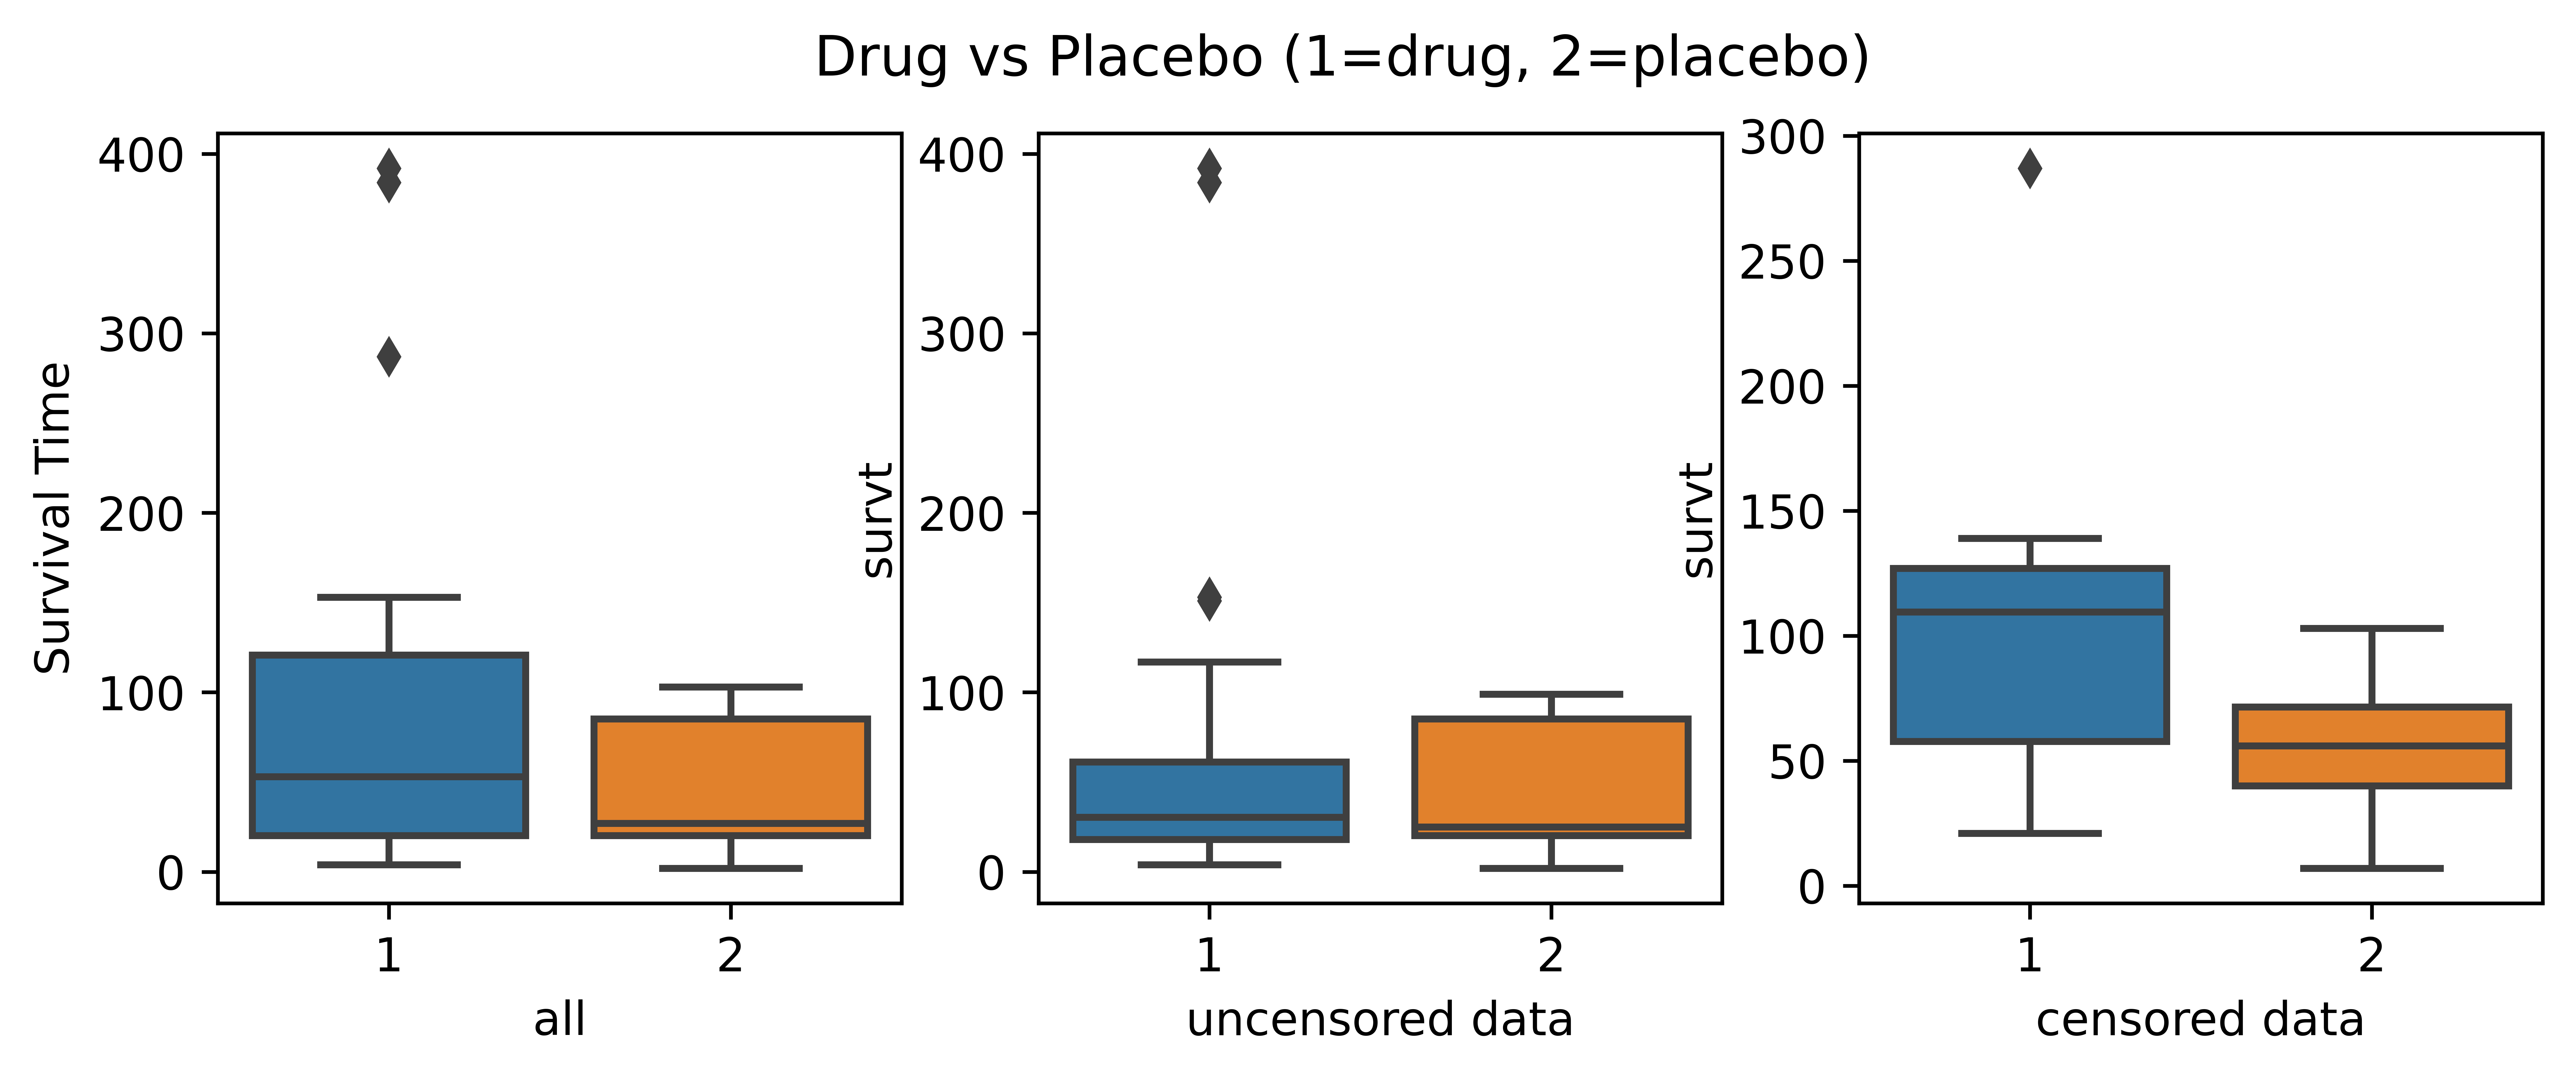
\includegraphics[width=0.999\linewidth]{img/boxplot_drug_vs_placebo_BOTH}
		\caption[Boxplot doby dožití]{Boxplot doby dožití (nalevo - celá analyzovaná skupina, uprostřed - pouze pro necensorovaná data, napravo - pouze pro censorovaná data)}
		\label{fig:boxplotdrugvsplacebo}
	\end{figure}

	Na Obrázku~\ref{fig:boxplotdrugvsplacebo} jsou tři boxploty, ilustrující rozdělení pacientů léčených lékem a placebem mezi censorovanými\footnote{V kontextu spolehlivostní analýzy censorované pozorování je neúplné nebo ne zcela pozorované měření. V tomto případě censorovaná pozorování jsou například pacienti, kteří přežili po celou dobu experimentu (a tedy okamžik úmrtí nebyl zaznamenán) nebo ukončili léčbu předčasně. Necensorovaná pozorování představují pacienty, jejichž úmrtí bylo pozorováno před koncem experimentu.} a necensorovanými případy. 
	Na všech třech boxplotech je vidět, že střední hodnota doby přežití je u pacientů léčených lékem vyšší, než u pacientů léčených placebem. 
	 
	Mezi skutečně léčenými pacienty je několik outlierů s výrazně nadprůměrnou dobou dožití. Může se jednat o případy, pro které testovaný lék je obzvláště účinný nebo se jedná pouze o přirozenou výjimku. Skutečnost, že taková odlehlá pozorování jsou pouze v případě léku a pouze na jednu stranu od průměru, napovídá k první variantě.
	
	Na Obrázku~\ref{fig:pairplot_my_data} je základní vizualizace datasetu (barevně jsou odděleny podskupiny, tj. lék a placebo).
    Vizualizace je pomocí pairplotu, tj. mřížka grafů, kde řádky i sloupce představují jednotlivé proměnné (sloupce) v datech. Tedy pairplot odráží, jak vypadá závislost proměnných mezi sebou, a na diagonále jsou histogramy pro danou proměnnou.
	
	\begin{figure}[H]
		\centering
		\includegraphics[width=1.0\linewidth]{img/pairplot_my_data_huebytreat.png}
		\caption{Pairplot}
		\label{fig:pairplot_my_data}
	\end{figure}
	

	\section{Parametrické a neparametrické modely}
    %Cílem této práce je určit, zda použití daného léku významně ovlivnilo dobu přežití u pacientů v dané skupině. 
    Cílem této práce je najít vhodný model popisující ve zvolené skupině doby dožití pro pacienty, kterým byl podáván lék a pro pacienty, kterým bylo podáváno placebo. 
	Nyní se pokusíme najít nejlepší modely pro popis dat, tedy vytvoříme pro každou skupinu pacientů vlastní model. Nejprve vyzkoušíme pro každou podskupinu parametrický přístup, poté neparametrický a následně výsledné modely porovnáme.
	
	
	\subsection{Parametrické modely} \label{sec:parametric_all}
	Ke hledání vhodného parametrického modelu použijeme existující implementaci v knihovně \texttt{reliability}. 
	V Podsekcích~\ref{sec:parametric_drugs}~a~\ref{sec:parametric_placebo} jsou pokaždé uvedeny grafické výstupy funkce \texttt{Fit\_Everything} a stručná diskuze, vysvětlující volbu konkrétní hustoty.
	Funkce \texttt{Fit\_Everything} proloží poskytnutá data pomocí 15 předdefinovaných hustot a pro každou odhadne hodnoty parametrů. Následně vykreslí PP ploty a probability ploty pro každý model (\uvoz{fit}).
	
	
	\subsubsection{Pacienti léčení lékem} \label{sec:parametric_drugs}
	
	\begin{figure}[H]
		\centering
		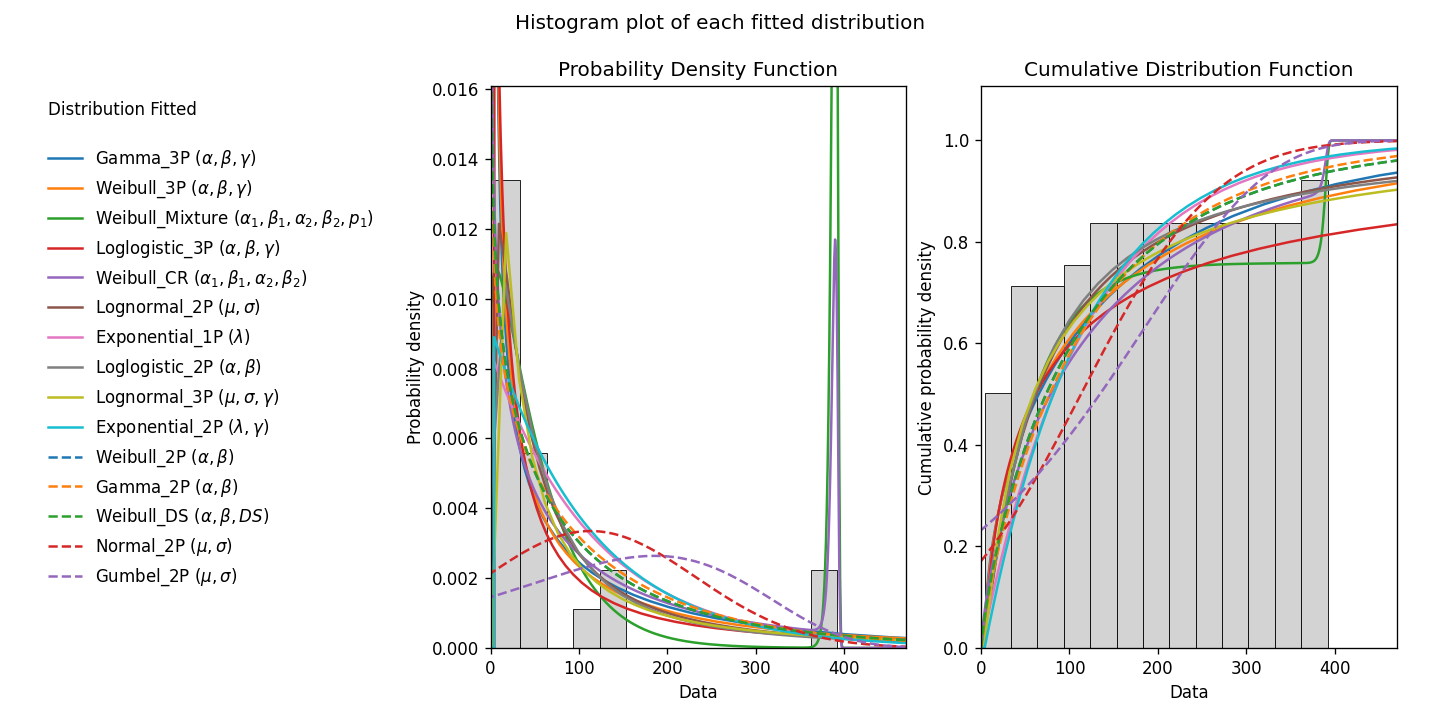
\includegraphics[width=0.9\linewidth]{img/fiteverything_drugs_histogram.png}
		\caption{Histogram a proložené hustoty}
		\label{fig:fit_everything_hist_drugs}
	\end{figure}

	\begin{figure}[H]
		\centering
		\includegraphics[width=1.0\linewidth]{img/fiteverything_drug_P_plots.png}
		\caption{P ploty pro jednotlivé modely}
		\label{fig:fit_everything_drug_P_plots}
	\end{figure}
	
	\begin{figure}[H]
		\centering
		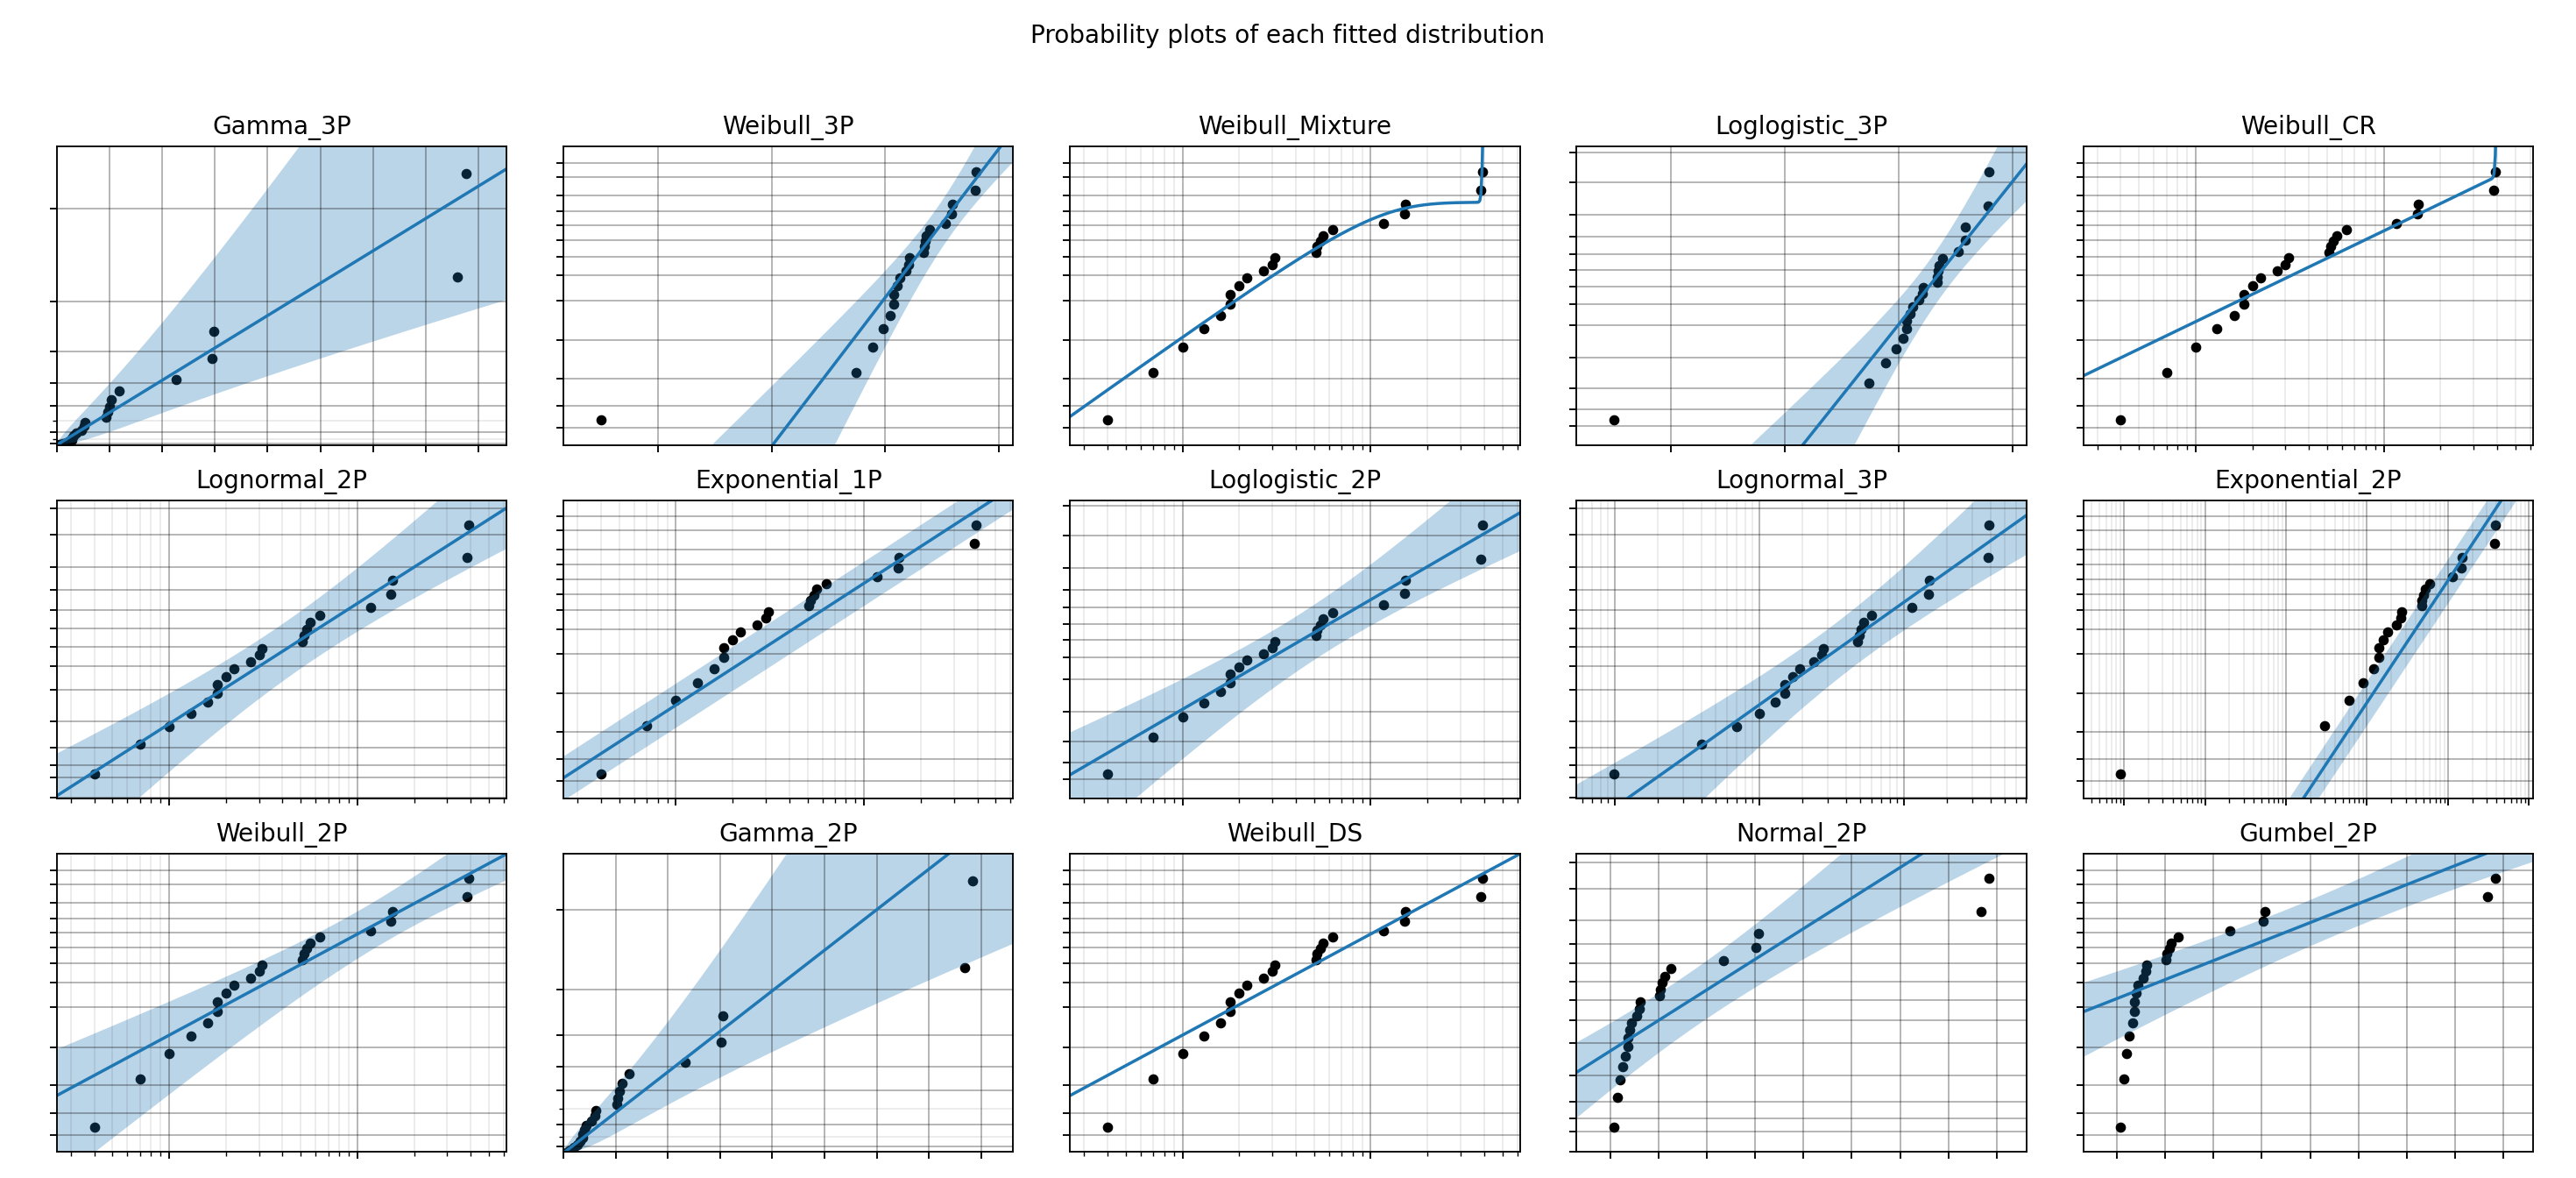
\includegraphics[width=0.8\linewidth]{img/fiteverything_drug_PP_plots.png}
		\caption{PP ploty pro jednotlivé modely}
		\label{fig:fit_everything_drug_PP_plots}
	\end{figure}
	
	V Tabulce~\ref{tab:fitall_output_parameters_tab} jsou shrnuty hodnoty odhadnutých parametrů a také hodnoty \texttt{log-likelihood}, \texttt{AIC} a \texttt{BIC}\footnote{Zde všechna čísla jsou zaokrouhlena na dvě desetinná místa.}.
	
%\begin{table}[H]
%	\tiny
%	\centering
%	\begin{tabular}{@{}|l|l|l|l|l|l|l|l|l|l|l|l|l|r|r|r|@{}}
%		\toprule
%		\textbf{Distribution} &
%		$\alpha$ &
%		$\beta$ &
%		$\gamma$ &
%		$\alpha_1$ &
%		$\beta_1$ &
%		$\alpha_2$ &
%		$\beta_2$ &
%		Prop. 1 &
%		DS &
%		$\mu$ &
%		$\sigma$ &
%		$\lambda$ &
%		\textbf{Log-like.} &
%		\textbf{AIC} &
%		\textbf{BIC} \\ \toprule
%		Gamma3P       & 270.72 & 0.50 & 4.00 &        &      &        &        &      &      &        &        &      & -120.39 & 247.71 & 250.99 \\ \midrule
%		Weibull3P     & 106.13 & 0.61 & 4.00 &        &      &        &        &      &      &        &        &      & -120.93 & 248.79 & 252.07 \\ \midrule
%		WeibullMixt.  &        &      &      & 56.57  & 1.10 & 389.96 & 116.37 & 0.76 &      &        &        &      & -118.04 & 248.57 & 253.08 \\ \midrule
%		Loglogistic3P & 57.80  & 0.78 & 4.00 &        &      &        &        &      &      &        &        &      & -122.66 & 252.25 & 255.53 \\ \midrule
%		WeibullCR     &        &      &      & 128.49 & 0.74 & 390.17 & 120.53 &      &      &        &        &      & -121.13 & 251.86 & 255.86 \\ \midrule
%		Lognormal2P   &        &      &      &        &      &        &        &      &      & 4.13   & 1.39   &      & -124.59 & 253.62 & 255.98 \\ \midrule
%		Exponential1P &        &      &      &        &      &        &        &      &      &        &        & 0.01 & -126.91 & 255.97 & 257.23 \\ \midrule
%		Loglogistic2P & 60.37  & 1.19 &      &        &      &        &        &      &      &        &        &      & -125.30 & 255.04 & 257.39 \\ \midrule
%		Lognormal3P   &        &      & 3.00 &        &      &        &        &      &      & 4.02   & 1.63   &      & -123.98 & 254.87 & 258.15 \\ \midrule
%		Exponential2P &        &      & 4.00 &        &      &        &        &      &      &        &        & 0.01 & -125.87 & 256.18 & 258.54 \\ \midrule
%		Weibull2P     & 114.41 & 0.83 &      &        &      &        &        &      &      &        &        &      & -126.20 & 256.85 & 259.21 \\ \midrule
%		Gamma2P       & 153.69 & 0.80 &      &        &      &        &        &      &      &        &        &      & -126.49 & 257.43 & 259.79 \\ \midrule
%		WeibullDS     & 114.41 & 0.83 &      &        &      &        &        &      & 1.00 &        &        &      & -126.20 & 259.33 & 262.61 \\ \midrule
%		Normal2P      &        &      &      &        &      &        &        &      &      & 112.97 & 119.09 &      & -141.89 & 288.23 & 290.58 \\ \midrule
%		Gumbel2P      &        &      &      &        &      &        &        &      &      & 185.54 & 139.42 &      & -147.79 & 300.02 & 302.38 \\ \bottomrule
%	\end{tabular}
%	\caption{Odhady parametrů pro podskupinu pacientů léčených lékem}
%	\label{tab:fitall_output_parameters_tab}
%	\normalsize
%\end{table}

\begin{table}[H]
    \tiny
    \centering
    \begin{tabular}{|l|l|l|l|l|l|l|l|l|l|l|l|l|r|r|r|}
        \hline
        \textbf{Distribution} &
        $\alpha$ &
        $\beta$ &
        $\gamma$ &
        $\alpha_1$ &
        $\beta_1$ &
        $\alpha_2$ &
        $\beta_2$ &
        Prop.&
        DS &
        $\mu$ &
        $\sigma$ &
        $\lambda$ &
        \textbf{Log-like.} &
        \textbf{AIC} &
        \textbf{BIC} \\ \hline
        Gamma3P       & 270.72 & 0.50 & 4.00 &        &      &        &        &      &      &        &        &      & -120.39 & 247.71 & 250.99 \\ \hline
        Weibull3P     & 106.13 & 0.61 & 4.00 &        &      &        &        &      &      &        &        &      & -120.93 & 248.79 & 252.07 \\ \hline
        WeibullMixt.  &        &      &      & 56.57  & 1.10 & 389.96 & 116.37 & 0.76 &      &        &        &      & -118.04 & 248.57 & 253.08 \\ \hline
        Loglogistic3P & 57.80  & 0.78 & 4.00 &        &      &        &        &      &      &        &        &      & -122.66 & 252.25 & 255.53 \\ \hline
        WeibullCR     &        &      &      & 128.49 & 0.74 & 390.17 & 120.53 &      &      &        &        &      & -121.13 & 251.86 & 255.86 \\ \hline
        Lognormal2P   &        &      &      &        &      &        &        &      &      & 4.13   & 1.39   &      & -124.59 & 253.62 & 255.98 \\ \hline
        Exponential1P &        &      &      &        &      &        &        &      &      &        &        & 0.01 & -126.91 & 255.97 & 257.23 \\ \hline
        Loglogistic2P & 60.37  & 1.19 &      &        &      &        &        &      &      &        &        &      & -125.30 & 255.04 & 257.39 \\ \hline
        Lognormal3P   &        &      & 3.00 &        &      &        &        &      &      & 4.02   & 1.63   &      & -123.98 & 254.87 & 258.15 \\ \hline
        Exponential2P &        &      & 4.00 &        &      &        &        &      &      &        &        & 0.01 & -125.87 & 256.18 & 258.54 \\ \hline
        Weibull2P     & 114.41 & 0.83 &      &        &      &        &        &      &      &        &        &      & -126.20 & 256.85 & 259.21 \\ \hline
        Gamma2P       & 153.69 & 0.80 &      &        &      &        &        &      &      &        &        &      & -126.49 & 257.43 & 259.79 \\ \hline
        WeibullDS     & 114.41 & 0.83 &      &        &      &        &        &      & 1.00 &        &        &      & -126.20 & 259.33 & 262.61 \\ \hline
        Normal2P      &        &      &      &        &      &        &        &      &      & 112.97 & 119.09 &      & -141.89 & 288.23 & 290.58 \\ \hline
        Gumbel2P      &        &      &      &        &      &        &        &      &      & 185.54 & 139.42 &      & -147.79 & 300.02 & 302.38 \\ \hline
    \end{tabular}
    \caption{Odhady parametrů pro podskupinu pacientů léčených lékem}
    \label{tab:fitall_output_parameters_tab}
    \normalsize
\end{table}

	Na základě vizuálního vyhodnocení P-plotů a PP-plotů (Obr.~\ref{fig:fit_everything_drug_P_plots} a Obr.~\ref{fig:fit_everything_drug_PP_plots}) 
	je vidět, že oba modely (\texttt{logNormal 2P} a \texttt{Gamma 3P}) popisují data podobně dobře, a to i ve srovnání s neparametrickými metodami Kaplan-Meiera a Nelson-Aalena (viz Podsekce~\ref{sec:non_parametric_all}), a tedy zvolíme jednodušší model -- dvouparametrickou lognormální hustotu s parametry $\mu = 4.02$ a $\sigma = 1.63$.
    
    (V následujících sekcích ověříme shodu zvoleného parametrického modelu s neparametrickými odhady.)
	
	
	\subsubsection{Pacienti léčení placebem} \label{sec:parametric_placebo}
	
    V této sekci hledáme stejným postupem parametrický model pro podskupinu pacientů s placebem.
	\begin{figure}[H]
		\centering
		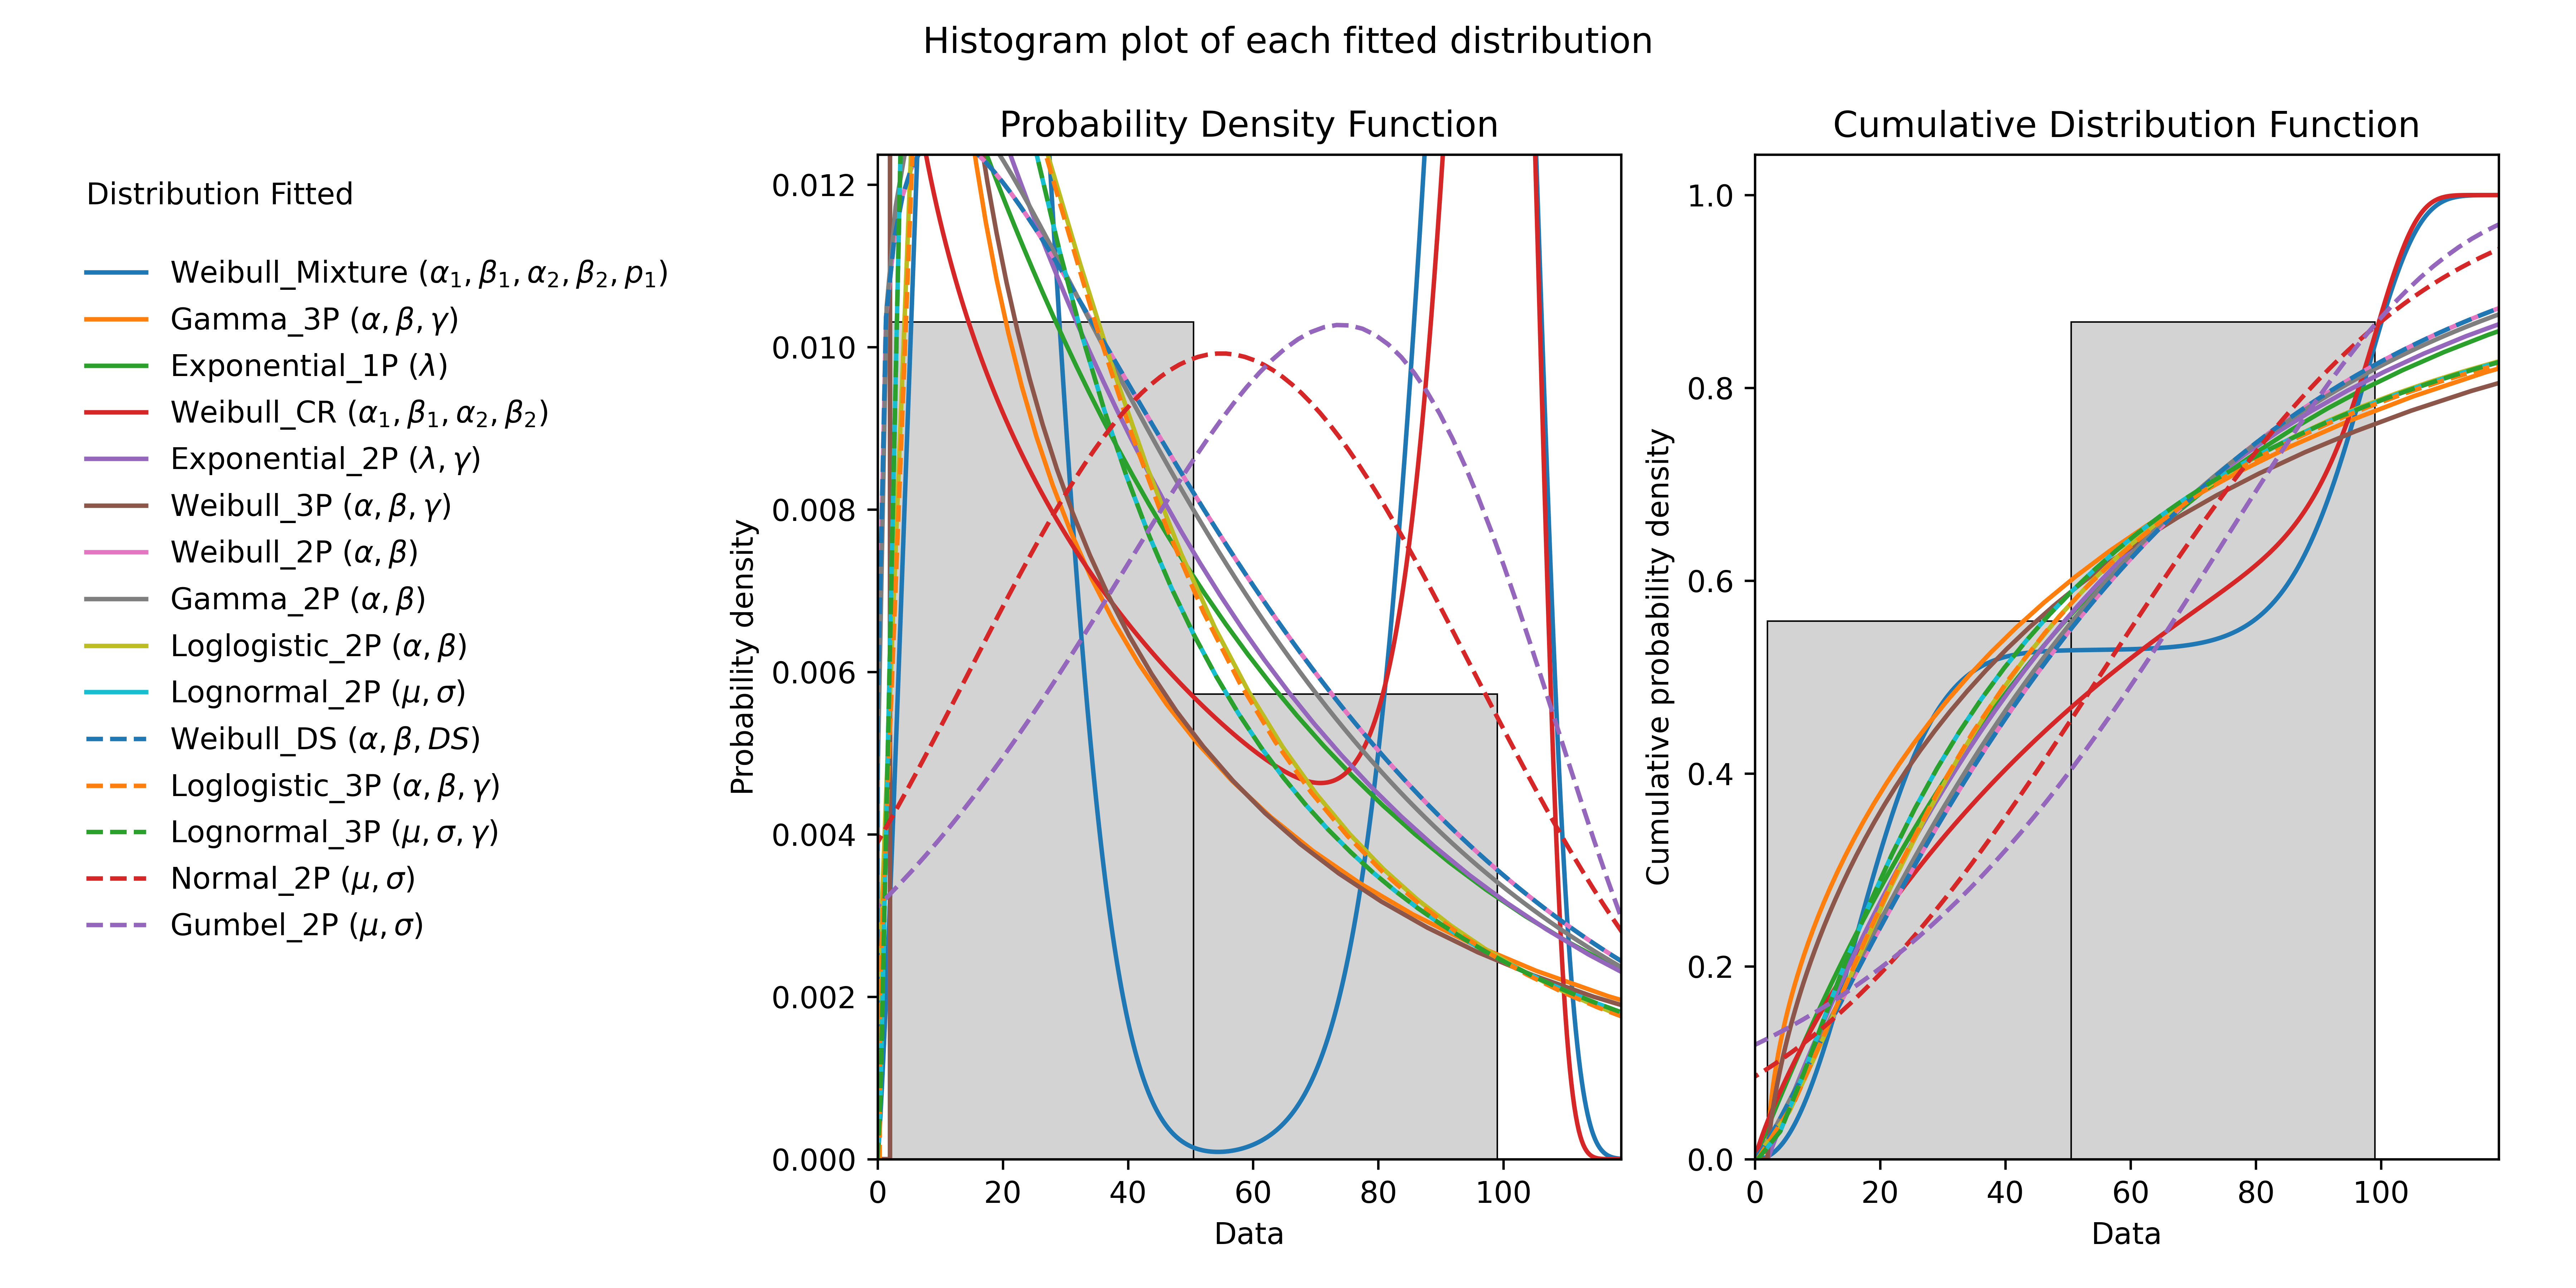
\includegraphics[width=0.8\linewidth]{img/fiteverything_placebo_histogram.png}
		\caption{Histogram a proložené hustoty}
		\label{fig:fit_everything_hist_placebo}
	\end{figure}

	\begin{figure}[H]
		\centering
		\includegraphics[width=1.0\linewidth]{img/fiteverything_placebo_P_plots.png}
		\caption{Probability ploty pro jednotlivé modely}
		\label{fig:fit_everything_placebo_P_plots}
	\end{figure}
    
	\begin{figure}[H]
        \centering
        \includegraphics[width=0.8\linewidth]{img/fiteverything_placebo_PP_plots.png}
        \caption{PP ploty pro jednotlivé modely}
        \label{fig:fit_everything_placebo_PP_plots}
    \end{figure}
    
    Číselné hodnoty parametrů jsou opět uvedeny v tabulce.
    
   \begin{table}[H]
       \tiny
       \centering
       \begin{tabular}{|l|l|l|l|l|l|l|l|l|l|l|l|l|r|r|r|}
           \hline
           \textbf{Distribution} &
           $\alpha$ &
           $\beta$ &
           $\gamma$ &
           $\alpha_1$ &
           $\beta_1$ &
           $\alpha_2$ &
           $\beta_2$ &
           Prop.&
           DS &
           $\mu$ &
           $\sigma$ &
           $\lambda$ &
           \textbf{Log-like.} &
           \textbf{AIC} &
           \textbf{BIC} \\ \hline
           WeibullMixt. &        &      &      & 20.74 & 2.23 & 98.21  & 12.93 & 0.53 &      &       &       &      & -63.67 & 142.33 & 141.78 \\ \hline
           Gamma3P        & 118.42 & 0.55 & 2.00 &       &      &        &       &      &      &       &       &      & -68.45 & 144.61 & 145.56 \\ \hline
           Exponential1P  &        &      &      &       &      &        &       &      &      &       &       & 0.02 & -71.47 & 145.19 & 145.83 \\ \hline
           WeibullCR      &        &      &      & 86.32 & 0.86 & 100.28 & 17.23 &      &      &       &       &      & -67.42 & 145.91 & 146.40 \\ \hline
           Exponential2P  &        &      & 2.00 &       &      &        &       &      &      &       &       & 0.02 & -70.86 & 146.53 & 147.51 \\ \hline
           Weibull3P      & 57.46  & 0.69 & 2.00 &       &      &        &       &      &      &       &       &      & -69.48 & 146.67 & 147.62 \\ \hline
           Weibull2P      & 61.35  & 1.15 &      &       &      &        &       &      &      &       &       &      & -71.27 & 147.35 & 148.33 \\ \hline
           Gamma2P        & 49.03  & 1.21 &      &       &      &        &       &      &      &       &       &      & -71.31 & 147.42 & 148.41 \\ \hline
           Loglogistic2P  & 40.88  & 1.47 &      &       &      &        &       &      &      &       &       &      & -72.07 & 148.93 & 149.91 \\ \hline
           Lognormal2P    &        &      &      &       &      &        &       &      &      & 3.66  & 1.19  &      & -72.11 & 149.02 & 150.00 \\ \hline
           WeibullDS      & 61.35  & 1.15 &      &       &      &        &       &      & 1.00 &       &       &      & -71.27 & 150.26 & 151.22 \\ \hline
           Loglogistic3P  & 40.43  & 1.44 & 0.34 &       &      &        &       &      &      &       &       &      & -72.06 & 151.84 & 152.80 \\ \hline
           Lognormal3P    &        &      & 0.00 &       &      &        &       &      &      & 3.66  & 1.19  &      & -72.11 & 151.93 & 152.89 \\ \hline
           Normal2P       &        &      &      &       &      &        &       &      &      & 54.95 & 40.21 &      & -74.39 & 153.59 & 154.57 \\ \hline
           Gumbel2P       &        &      &      &       &      &        &       &      &      & 74.07 & 35.81 &      & -75.54 & 155.88 & 156.86 \\ \hline
       \end{tabular}
       \caption{Odhady parametrů pro podskupinu pacientů léčených placebem}
       \label{tab:fitall_output_parameters_tab_placebo}
       \normalsize
   \end{table}
    
    Pro podskupinu pacientů léčených placebem jsme zvolili jednoparametrickou exponenciální hustotu s hodnotou parametru $\lambda = 0.0165$. Hustota \texttt{Gamma3P} popisuje data jen nepatrně lépe, zato ale se musí odhadovat 3 parametry místo 1. Volíme tedy jednodušší model.
    
    
	
	\subsection{Neparametrické modely} \label{sec:non_parametric_all}
	V Podsekcích~\ref{sec:non_parametric_drugs}~a~\ref{sec:non_parametric_placebo} jsou pro obě skupiny pacientů (tj. léčení lékem a léčení placebem) uvedeny odhady Kaplan-Meiera a Nelson-Aalena.
	Na grafech jsou pro porovnání vyneseny také vybrané parametrické odhady (viz Sekce~\ref{sec:parametric_all}).
	
	\subsubsection{Pacienti léčení lékem} \label{sec:non_parametric_drugs}
	Na Obrázku~\ref{fig:four_men_drugs} jsou \textit{survival function} (SF), \textit{cumulative distribution function} (CDF) a \textit{complementary hazard function} (CHF).
    
	\begin{figure}[H]
		\centering
		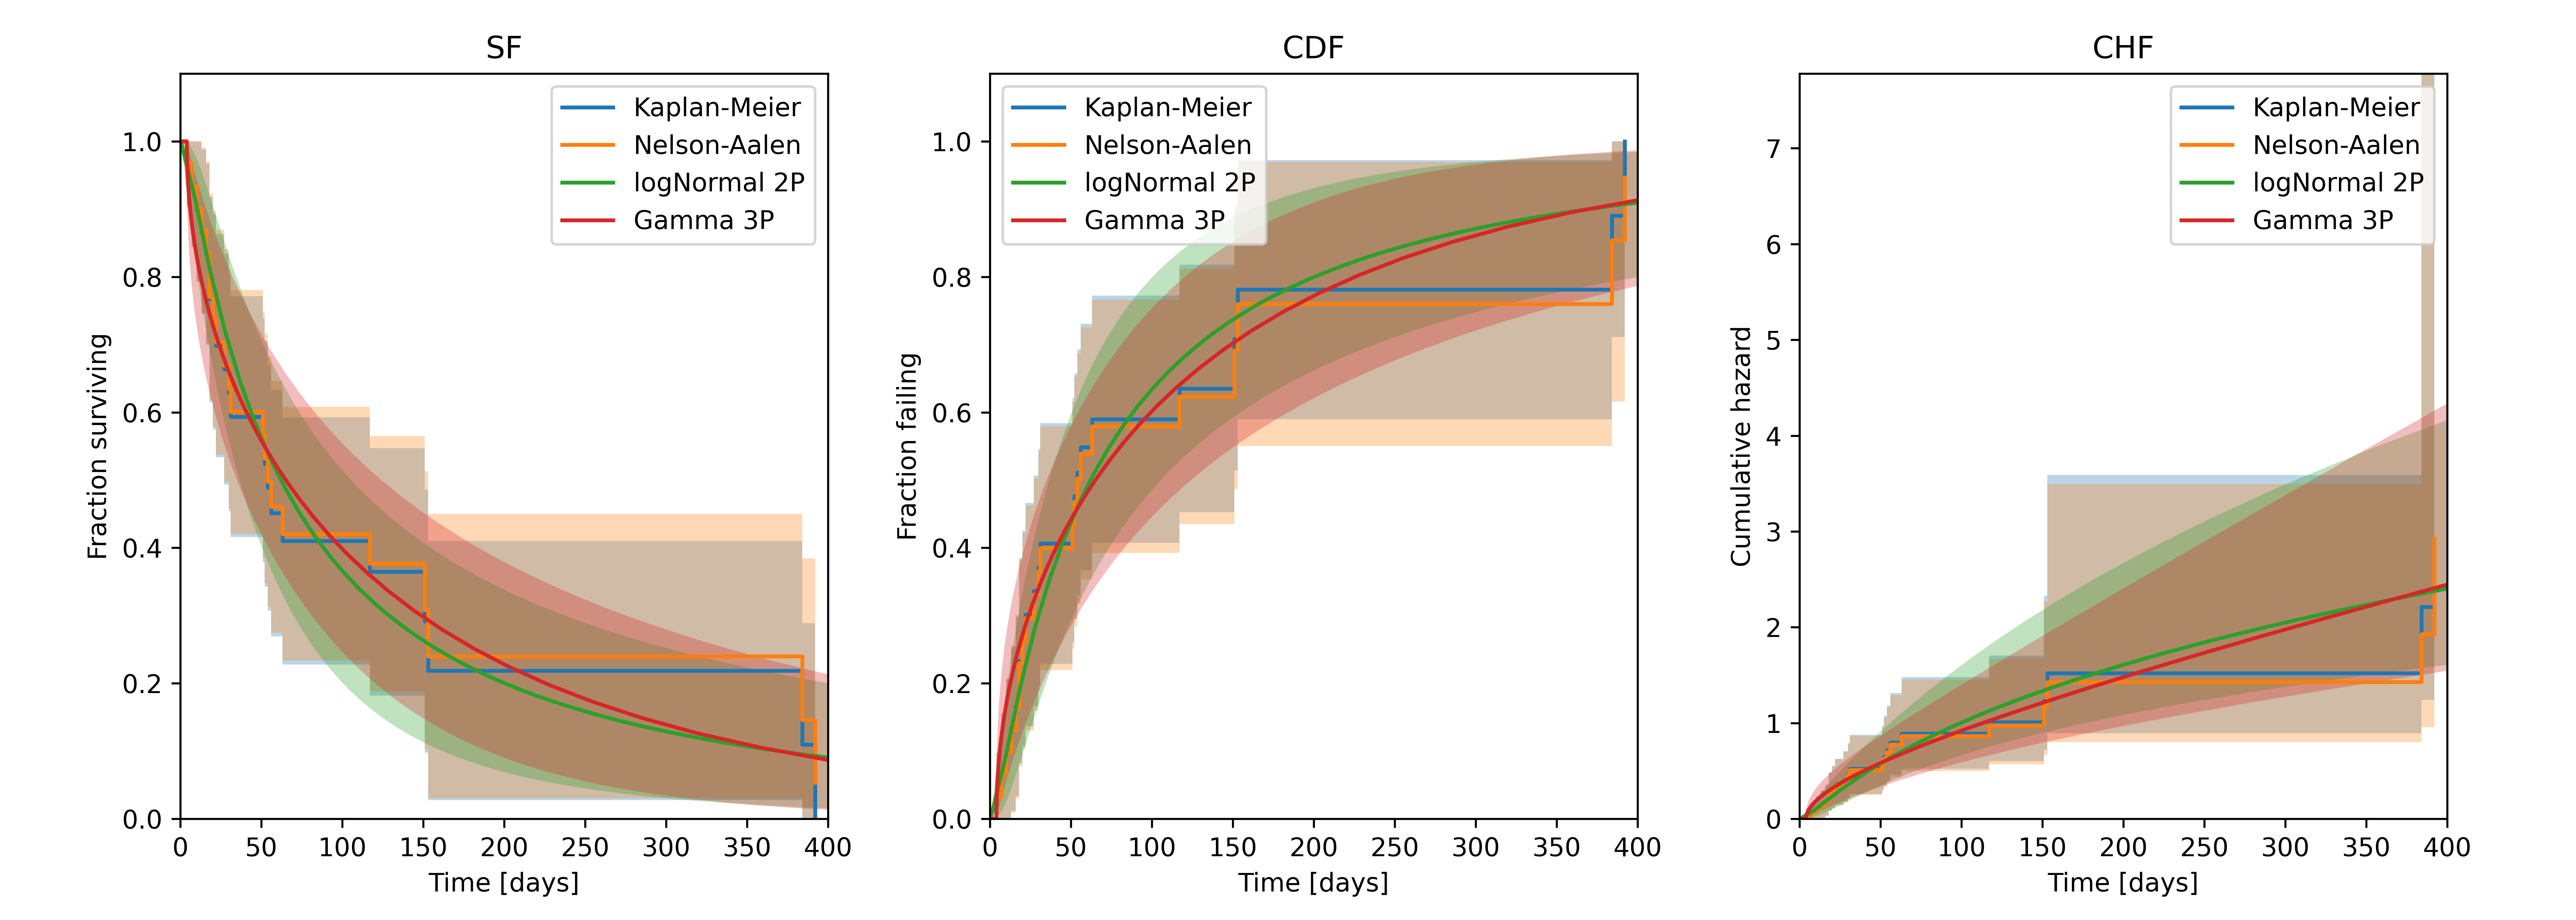
\includegraphics[width=0.9\linewidth]{img/four_men_drugs.png}
		\caption{SF, CDF a CHF pro odhad Nelson-Aalena a Kaplan-Meiera pro podskupinu pacientů, léčených lékem.}
		\label{fig:four_men_drugs}
	\end{figure}
    
    Na ose x je vynesen počet dnů do hodnoty 400, jelikož maximální hodnota \texttt{survt} pro pacienty léčené lékem je 392.
    
    Obrázek~\ref{fig:four_men_drugs_compared_to_parametrics} ilustruje shodu těchto neparametrických metod s parametrickými modely, zvolenými v předchozí sekci.
    
	\begin{figure}[H]
        \centering
        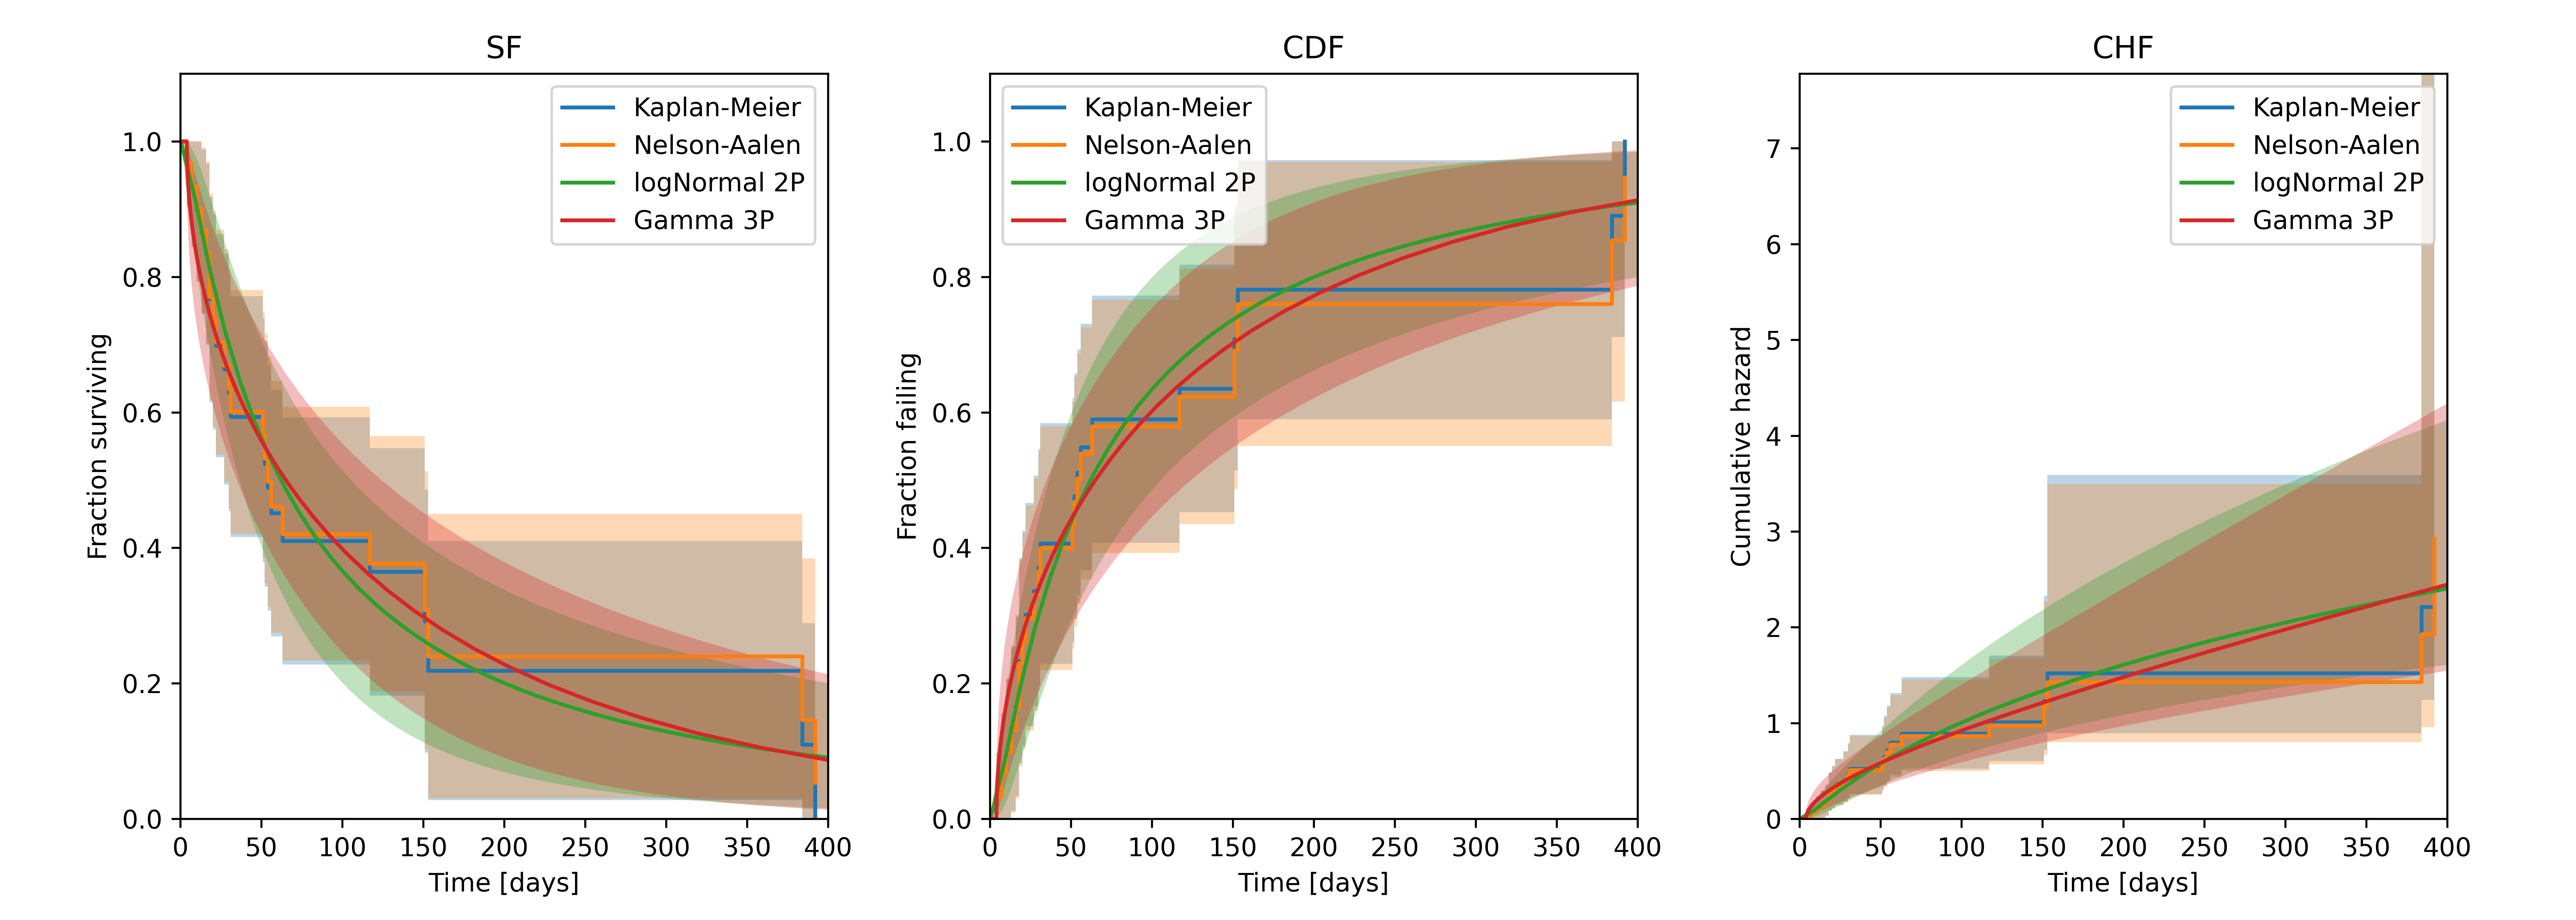
\includegraphics[width=0.9\linewidth]{img/four_men_drugs_compared_to_parametrics.png}
        \caption{SF, CDF a CHF - porovnání parametricky a neparametricky}
        \label{fig:four_men_drugs_compared_to_parametrics}
    \end{figure}

	
	\subsubsection{Pacienti léčení placebem} \label{sec:non_parametric_placebo}
	Opět SF, CDF a CHF pro podskupinu pacientů léčenou placebem.
    
	\begin{figure}[H]
		\centering
		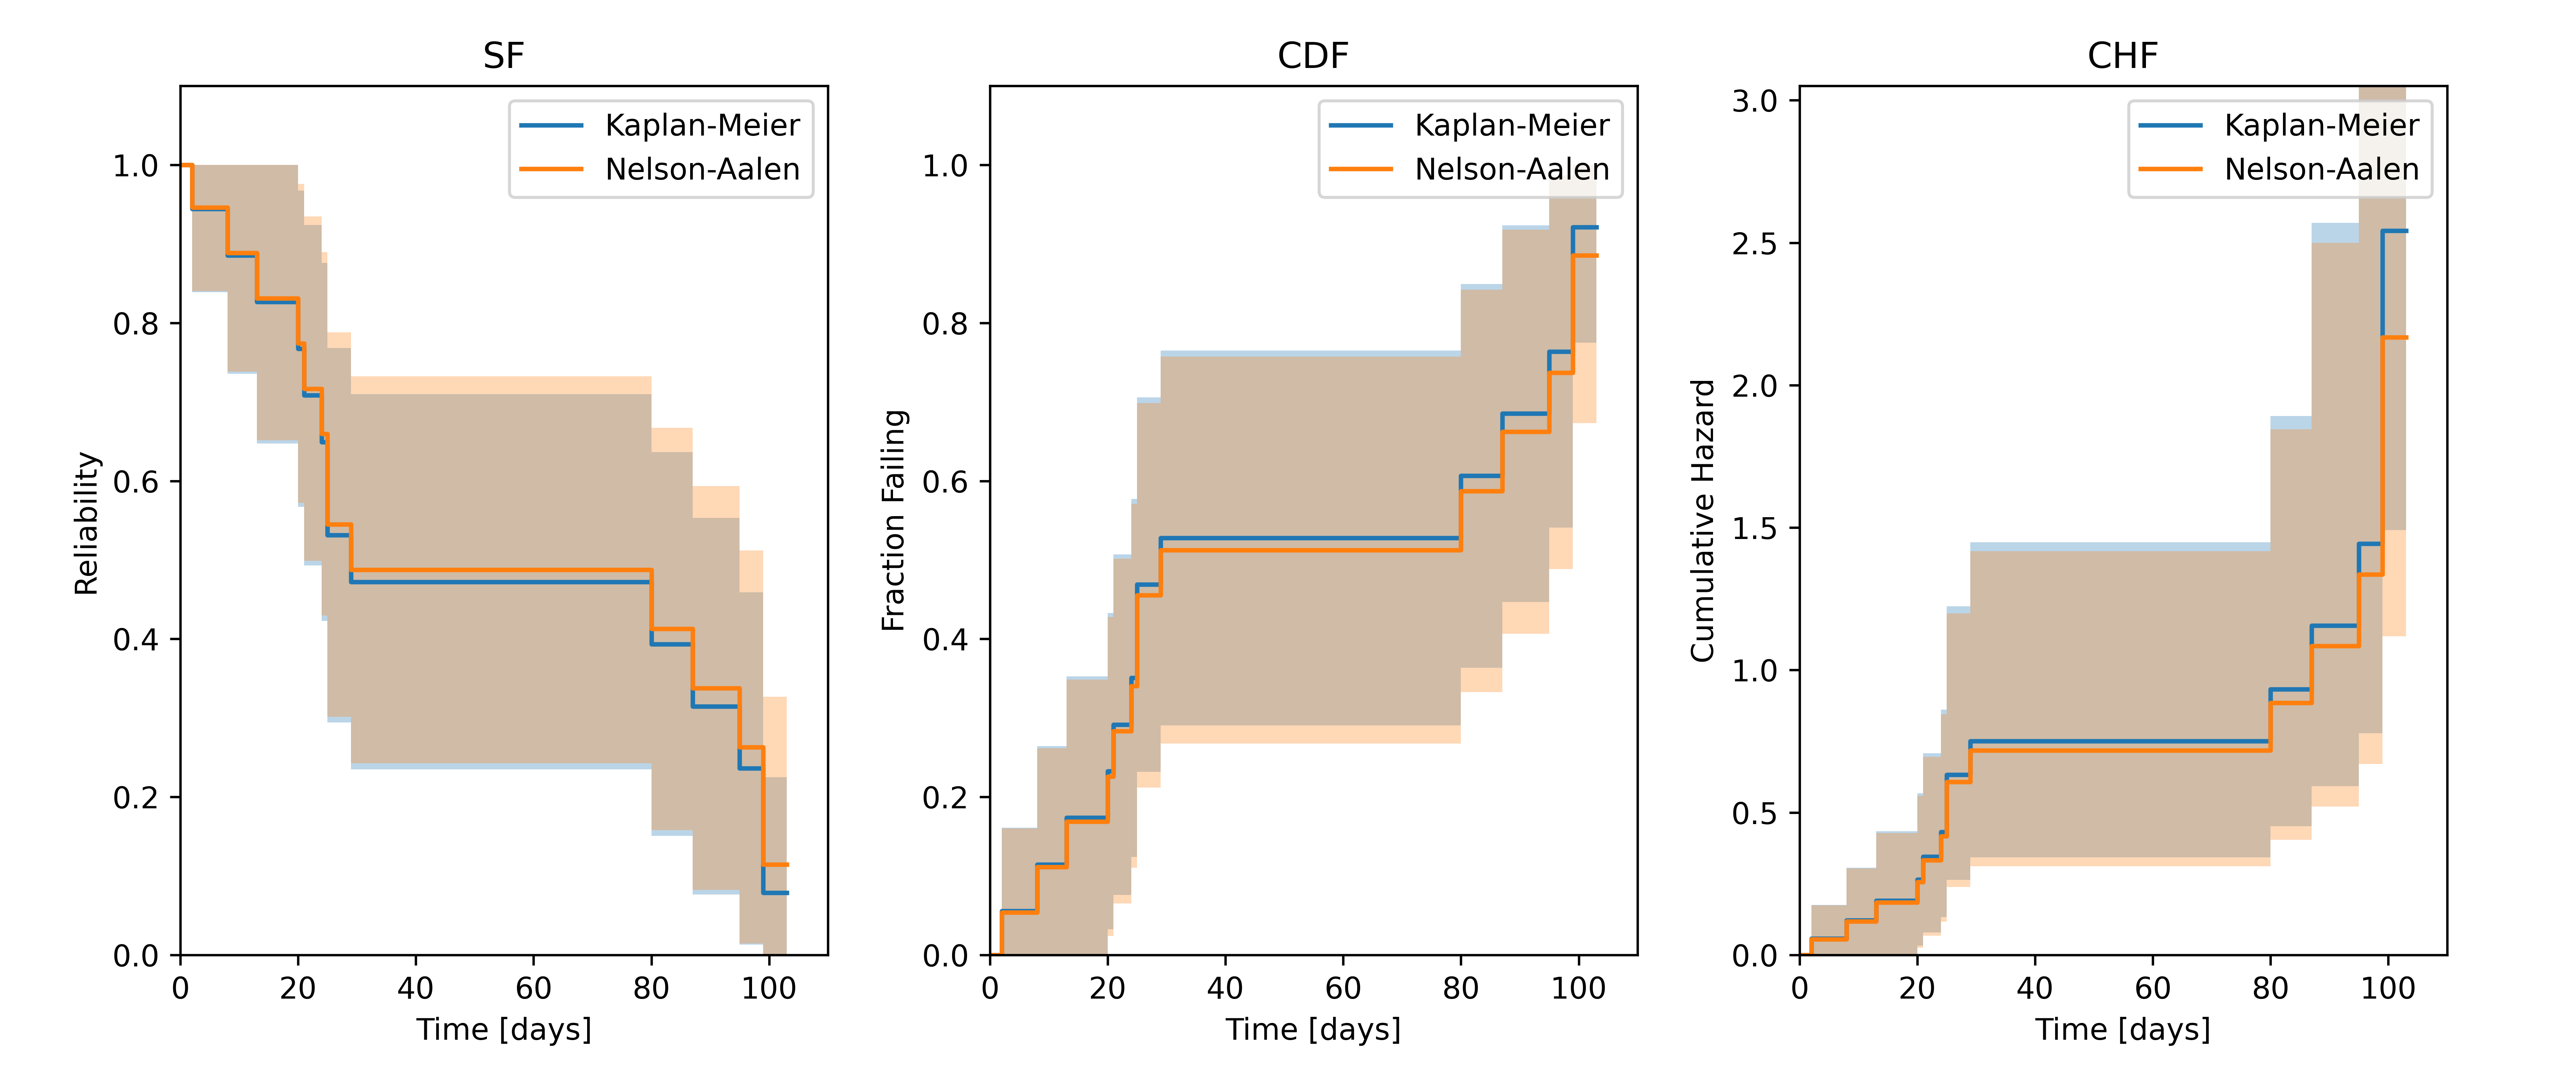
\includegraphics[width=0.9\linewidth]{img/four_men_placebo.png}
		\caption{SF, CDF a CHF pro odhad Nelson-Aalena a Kaplan-Meiera pro podskupinu pacientů, léčených placebem}
		\label{fig:four_men_placebo}
	\end{figure}

	\begin{figure}[H]
    	\centering
    	\includegraphics[width=0.9\linewidth]{img/four_men_placebo_compared_to_parametrics.png}
    	\caption{SF, CDF a CHF - porovnání parametricky a neparametricky}
    	\label{fig:four_men_placebo_comp_to_parametrics}
    \end{figure}
	
	Zde je počet dnů vynesen pouze do hodnoty 110, jelikož maximální hodnota \texttt{survt} pro pacienty léčené placebem je 103.
    
    Obrázek~\ref{fig:four_men_placebo_comp_to_parametrics} opět ukazuje shodu parametrických a neparametrických modelů.
	
	
	\section{Porovnání podskupin lék vs. placebo} \label{sec:comparison_drug_vs_placebo}
	V této sekci uvedeme porovnání modelů, sestavených v předchozích sekcích. Na Obrázku~\ref{fig:TTTplot} je TTTplot (total time in test), konstruovaný na základě Kaplan-Meiera. 
    Je vidět, že pacienti, dostávající placebo, umírali výrazně rychleji. Na grafu pacientů, léčených lékem (modrá barva) je mezi 150. a 360. dnem vidět plató - patrně lze říct, že u dosud přeživších se eskalace nemoci zastavila (lék zabral).

	\begin{figure}[H]
        \centering
        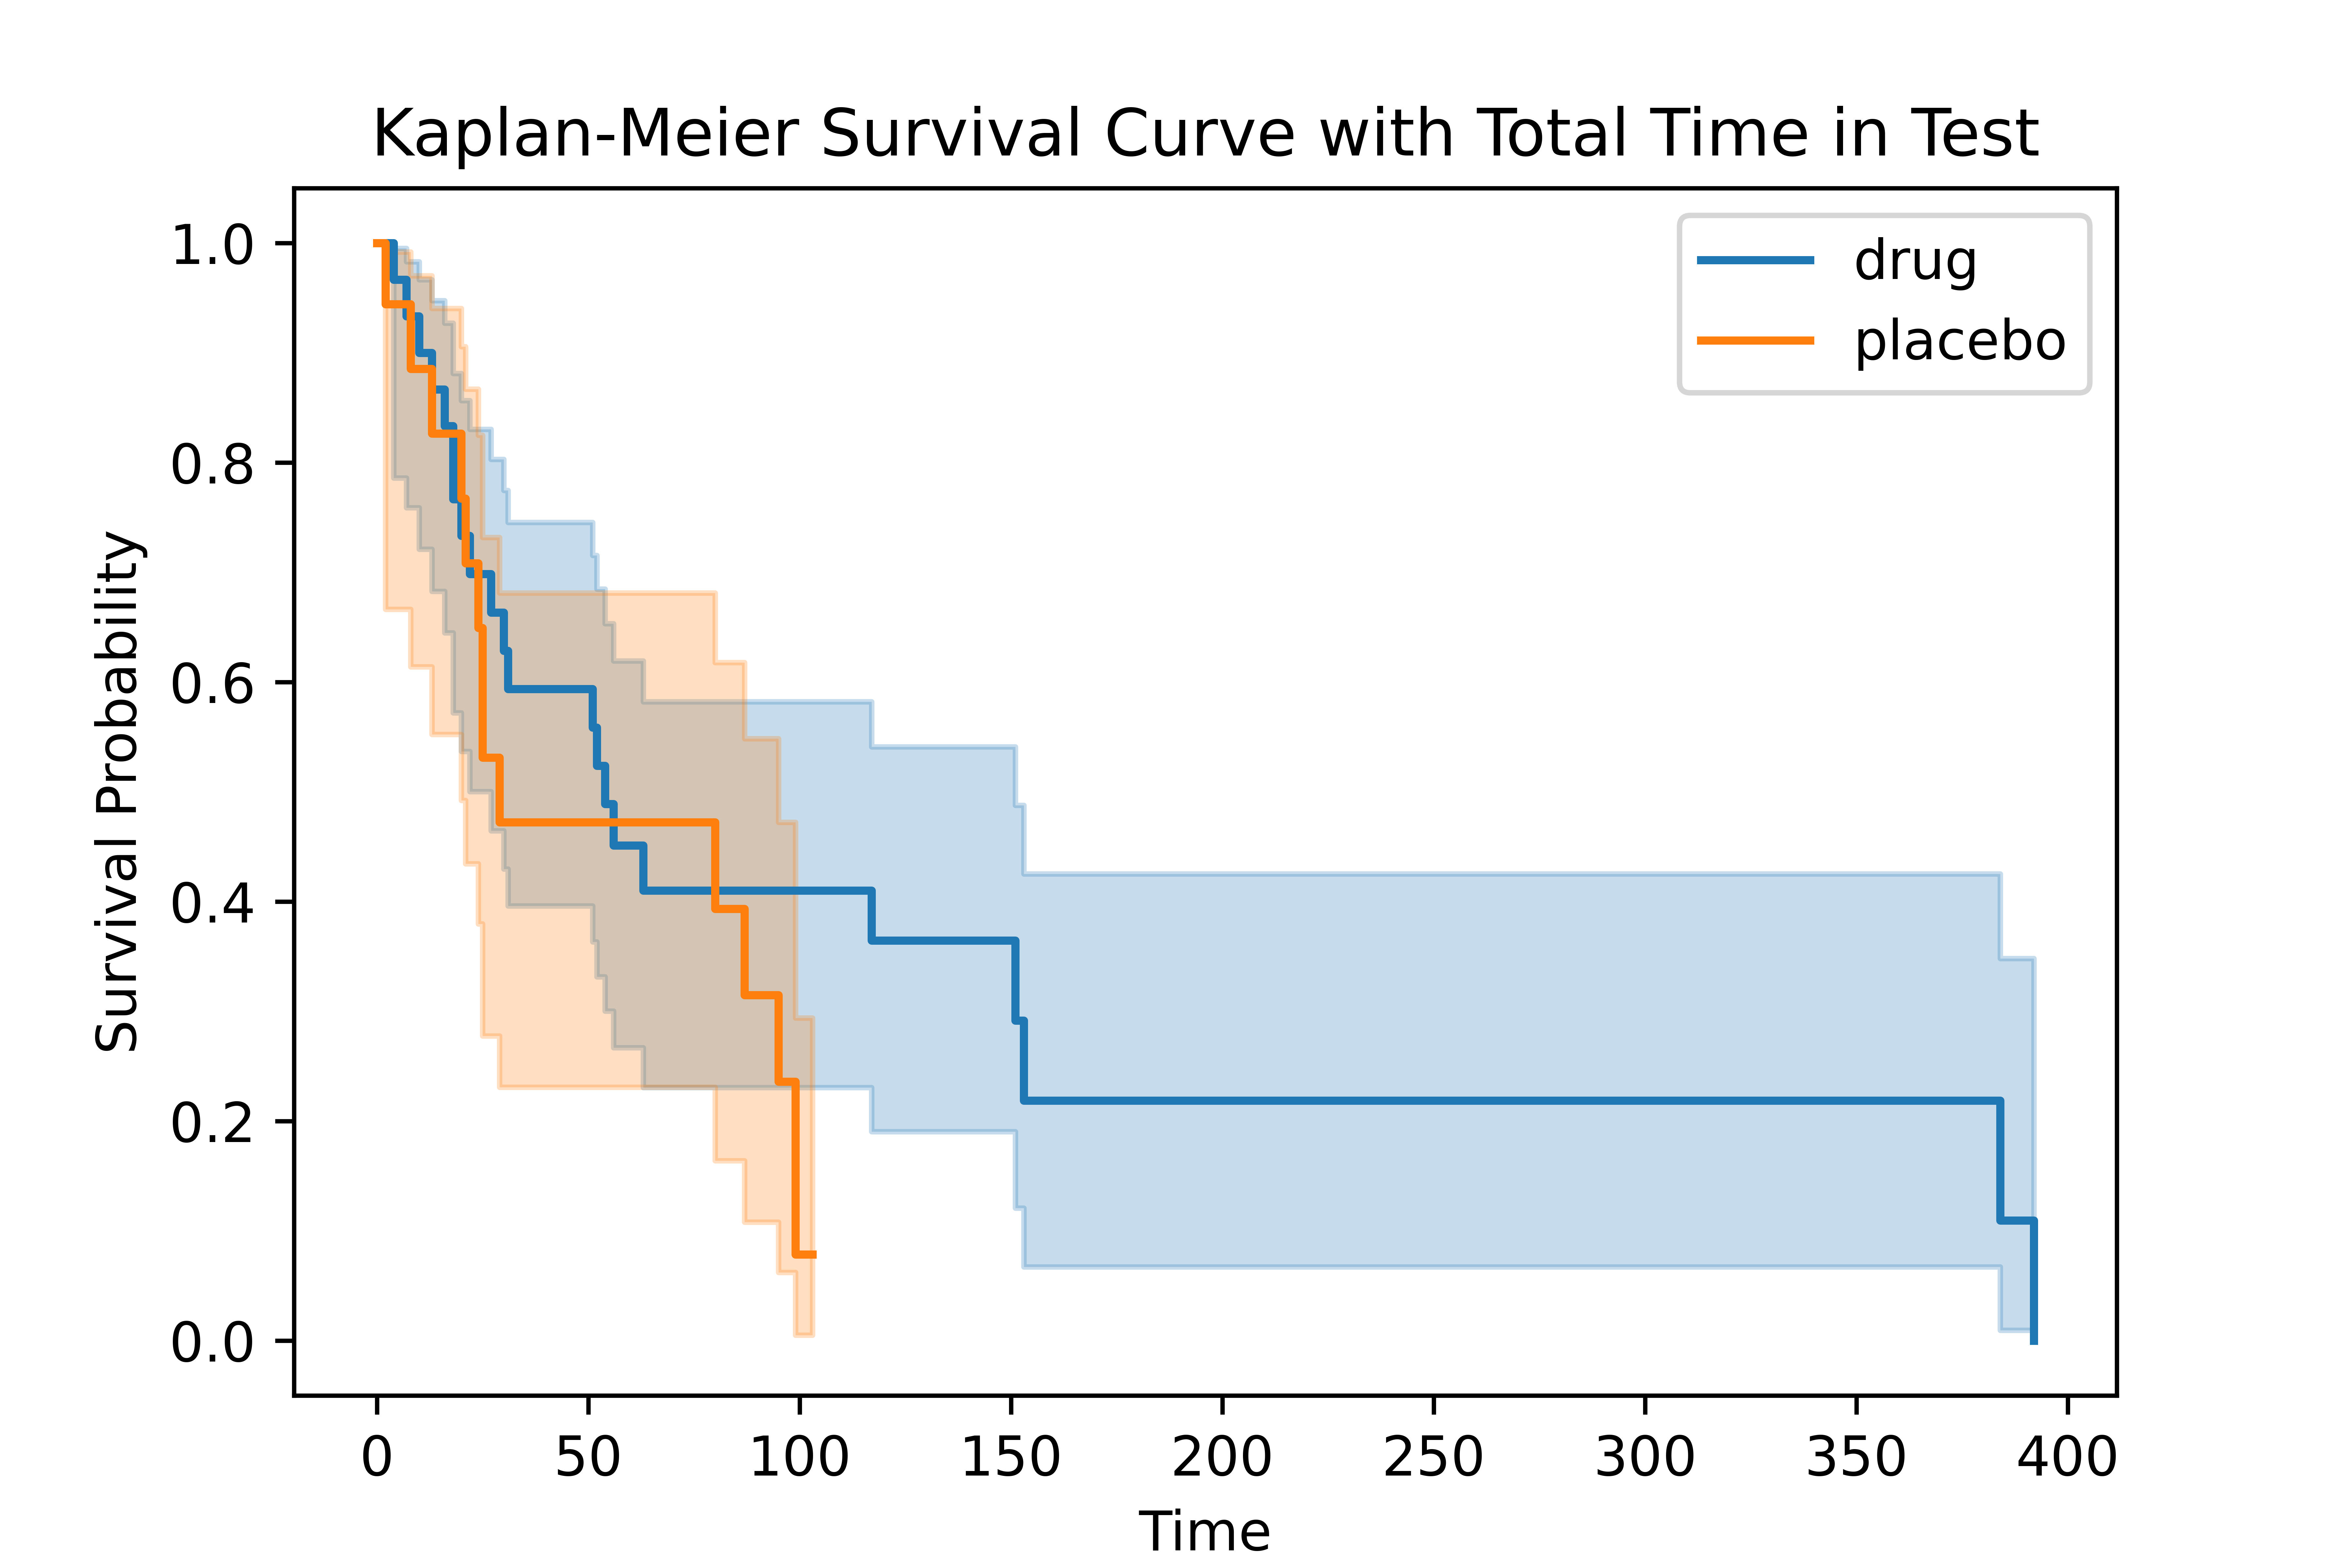
\includegraphics[width=0.5\linewidth]{img/TTTplot_using_KM.png}
        \caption{TTT plot (na základě Kaplan-Meiera)}
        \label{fig:TTTplot}
    \end{figure}
    
    Obrázek~\ref{fig:SF_for_parametric} (ukazující SF pro parametrické modely) je ve shodě s Obrázkem~\ref{fig:TTTplot}, tedy ilustruje o něco rychlejší (ve smyslu doby do úmrtí) průběh nemoci u pacientů, kteří dostávali placebo.
    
   	\begin{figure}[H]
        \centering
        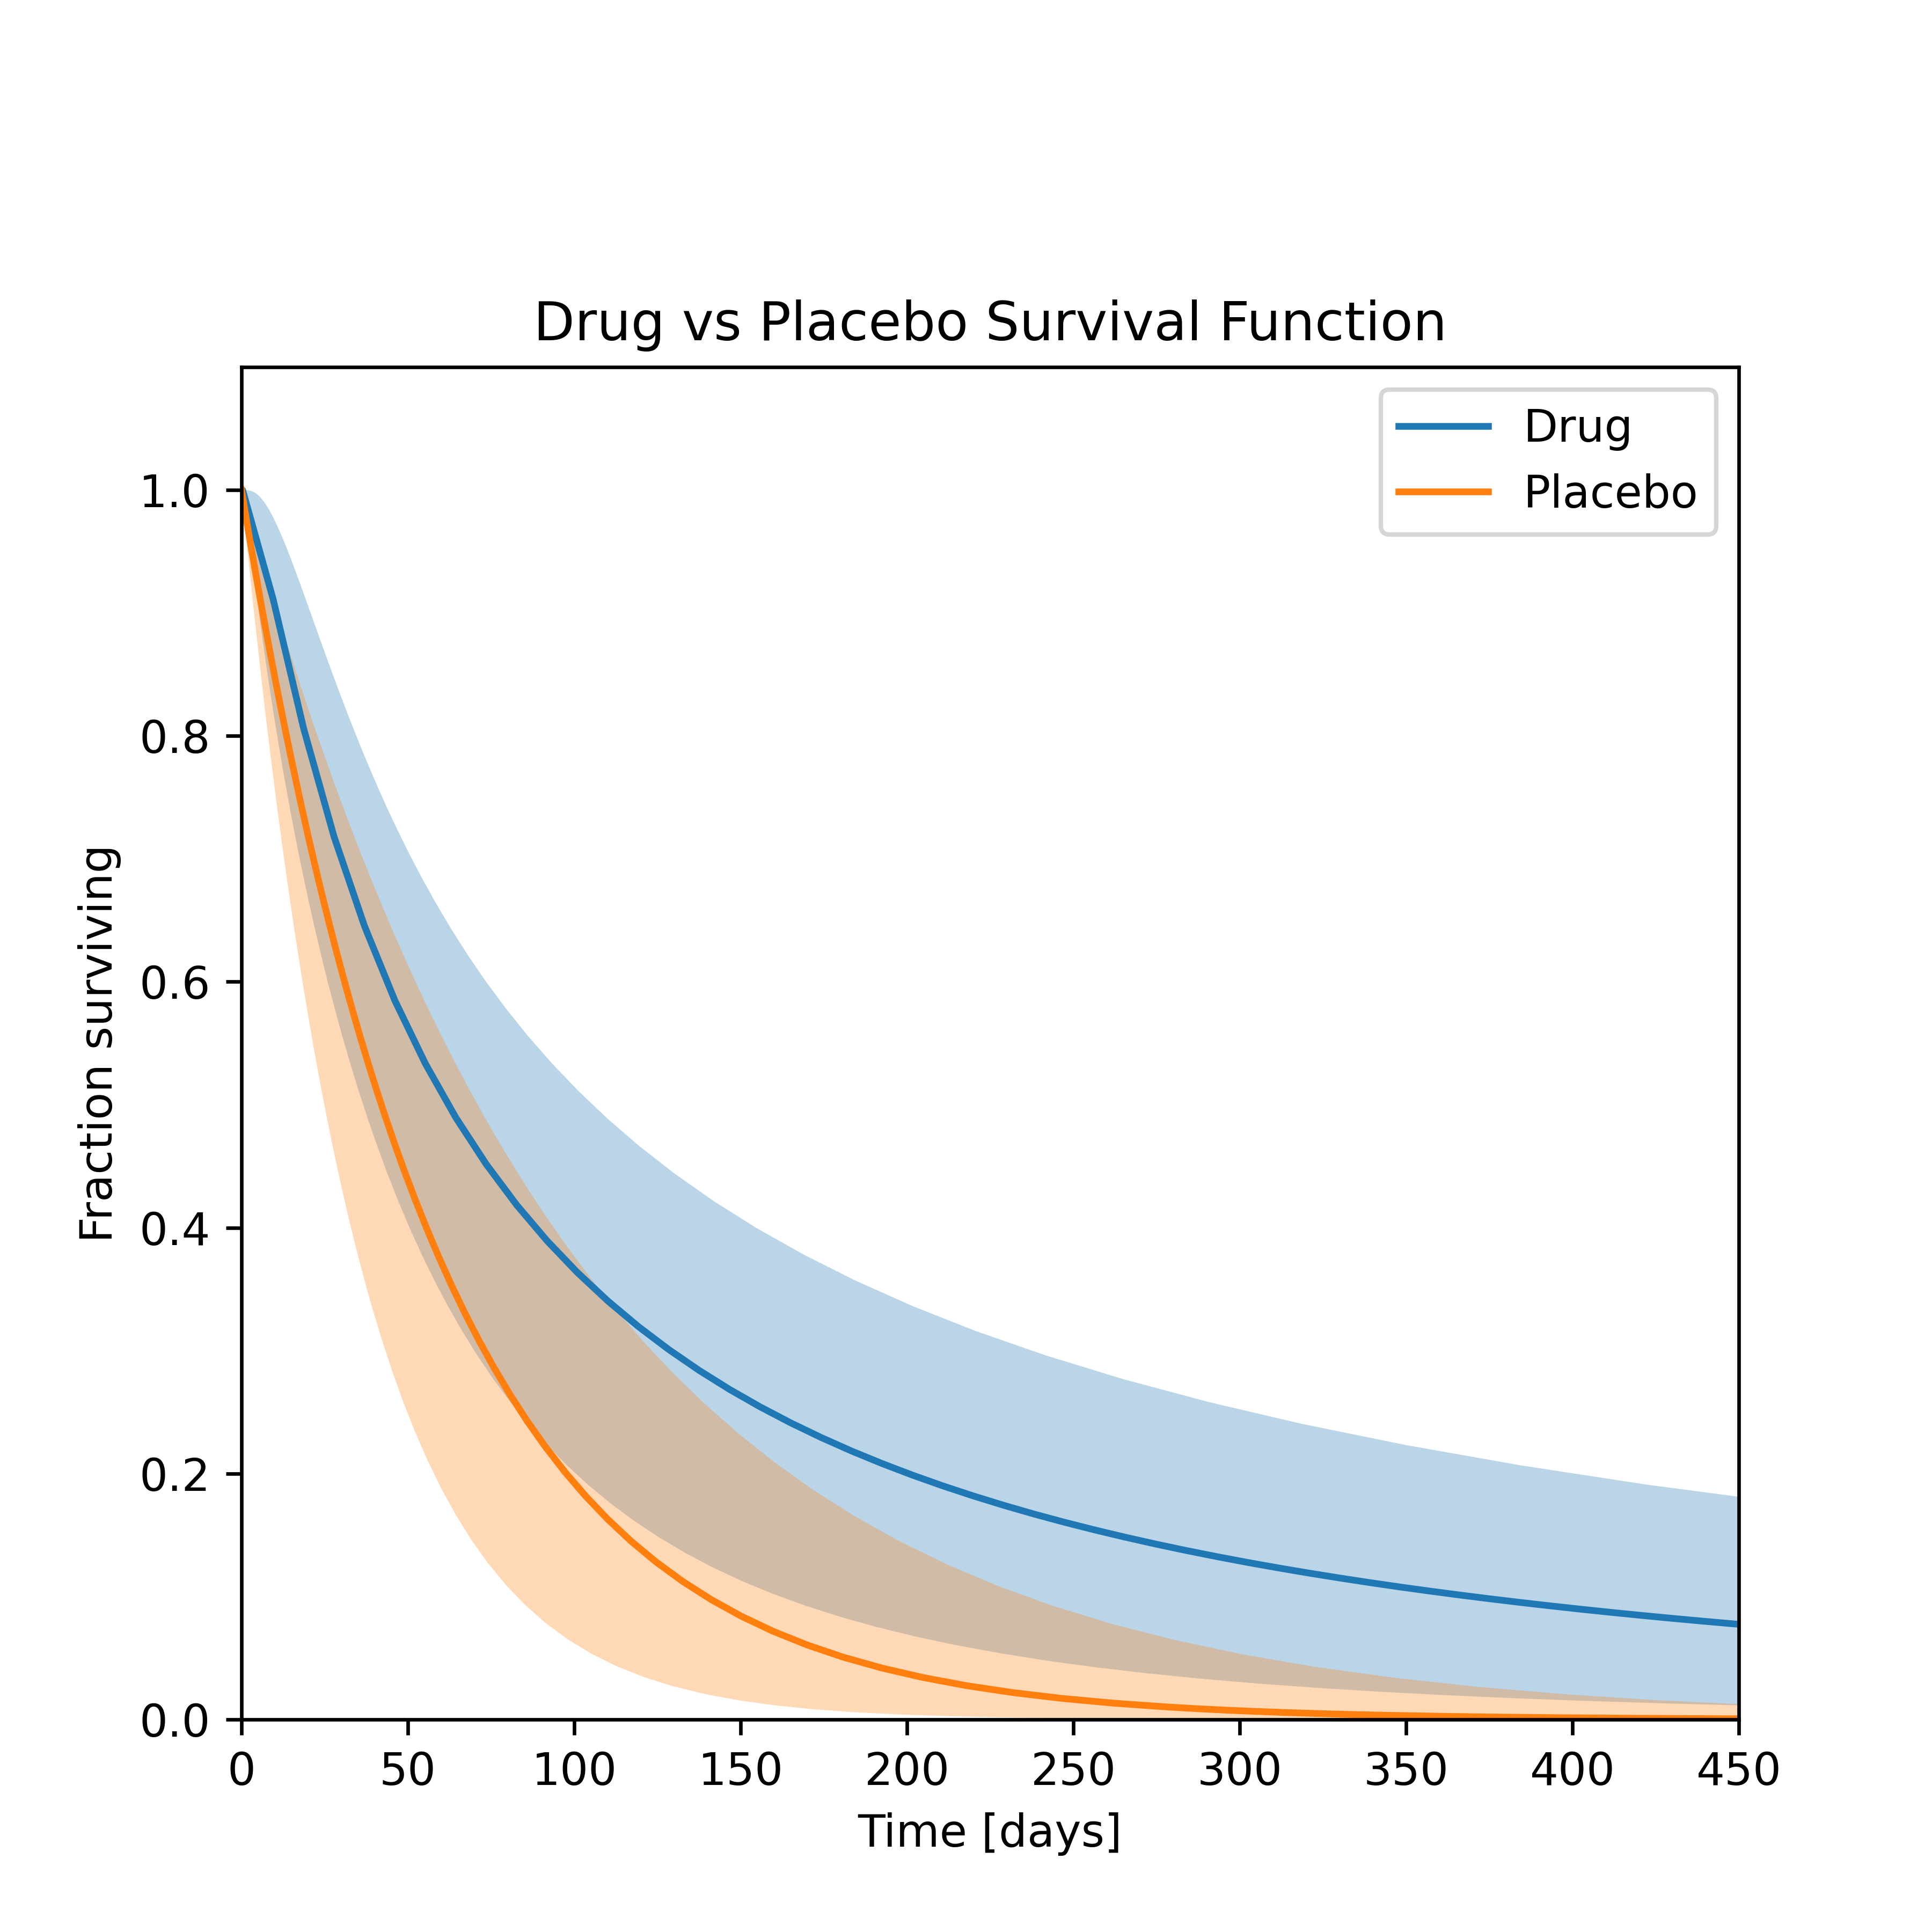
\includegraphics[width=0.5\linewidth]{img/survival_function_drug_vs_placebo_parametric.png}
        \caption{Průběh survival function pro vybrané parametrické modely.}
        \label{fig:SF_for_parametric}
    \end{figure}
    
   	\begin{figure}[H]
        \centering
        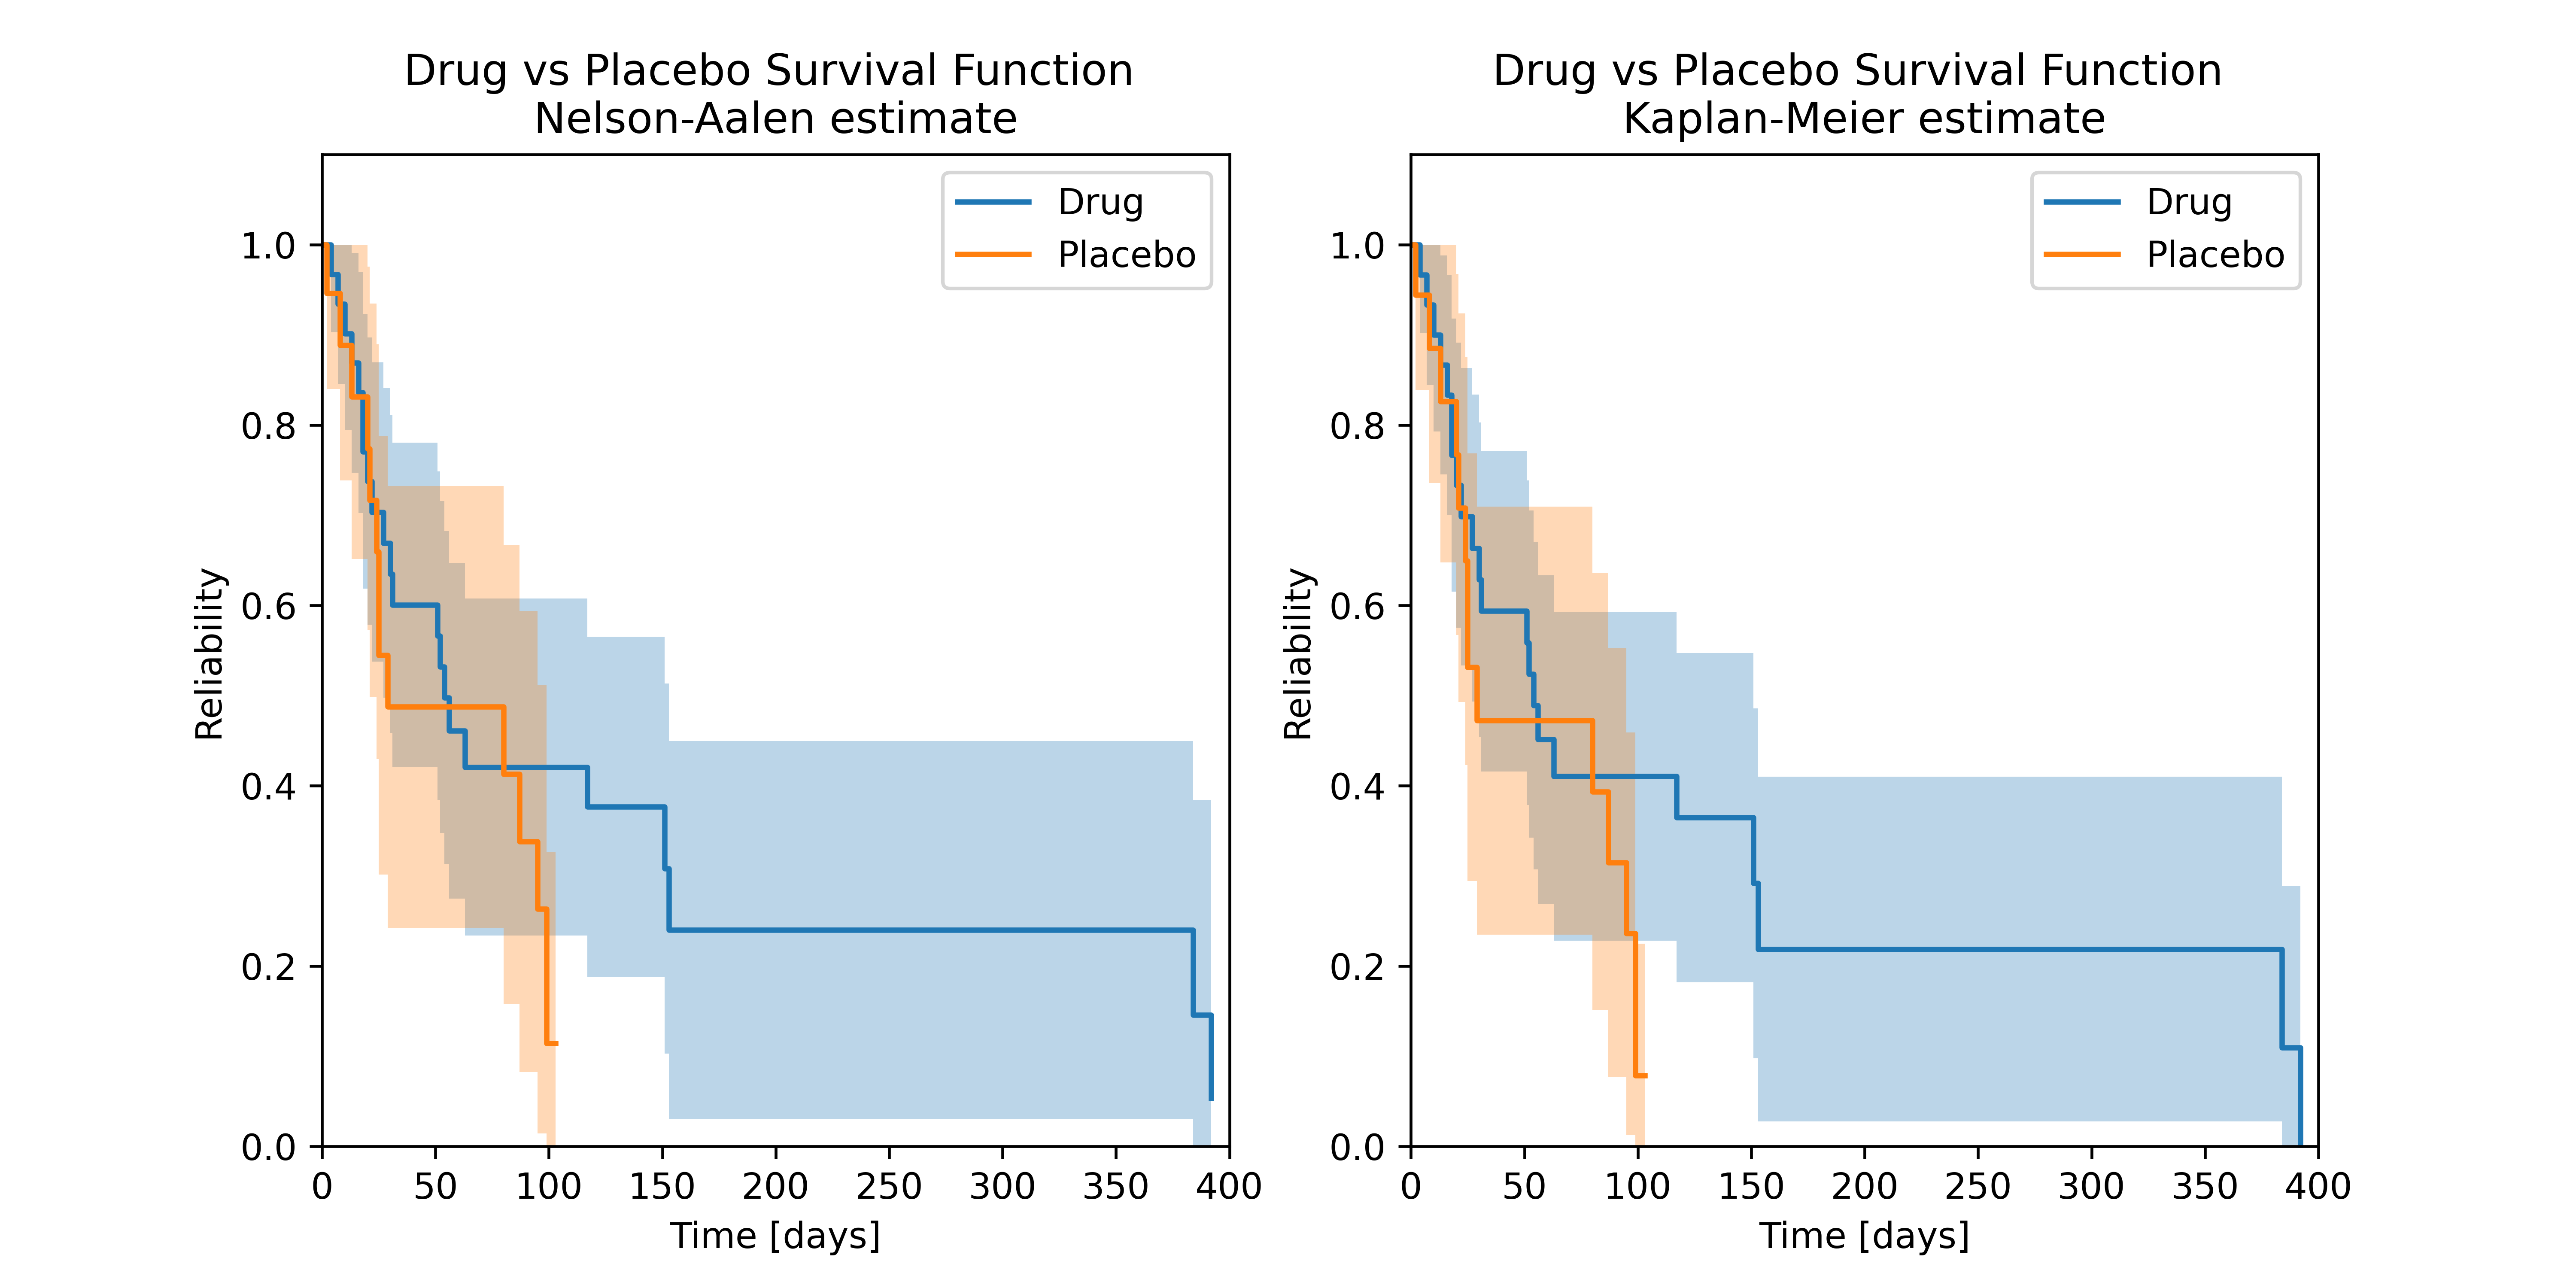
\includegraphics[width=0.9\linewidth]{img/survival_function_drug_vs_placebo_NON_parametric.png}
        \caption{Průběh survival function pro vybrané neparametrické modely (KM, NA)}
        \label{fig:SF_for_nonparametric}
    \end{figure}    
    
    \textbf{Poznámka k Obrázkům~\ref{fig:SF_for_parametric}~a~\ref{fig:SF_for_nonparametric}:} na první pohled lze říct, že SF pro pacienty s placebem od 100. dne léčby, získané parametrickým a neparametrickým přístupem, se neshodují. Je to vysvětlitelné tím, že po 100. dni již nebyla žádná další pozorování úmrtí, a tedy parametrický odhad může být nekvalitní.
    
    Na Obrázku~\ref{fig:HF_for_parametric} je průběh intenzity poruch pro dvě zvolené parametrické hustoty: lognormální o dvou parametrech (popisující podskupinu pacientů, léčených lékem) a exponenciální o jednom parametru (popisující podskupinu pacientů, léčených placebem).
    Pacienti s placebem mají \textit{constant failure rate}. U pacientů s lékem je vidět, že pokud pacient přežije prvních 30 dnů léčby, dále riziko úmrtí bude klesat. Lze tedy říct, že lék zabírá.
    
   	\begin{figure}[H]
        \centering
        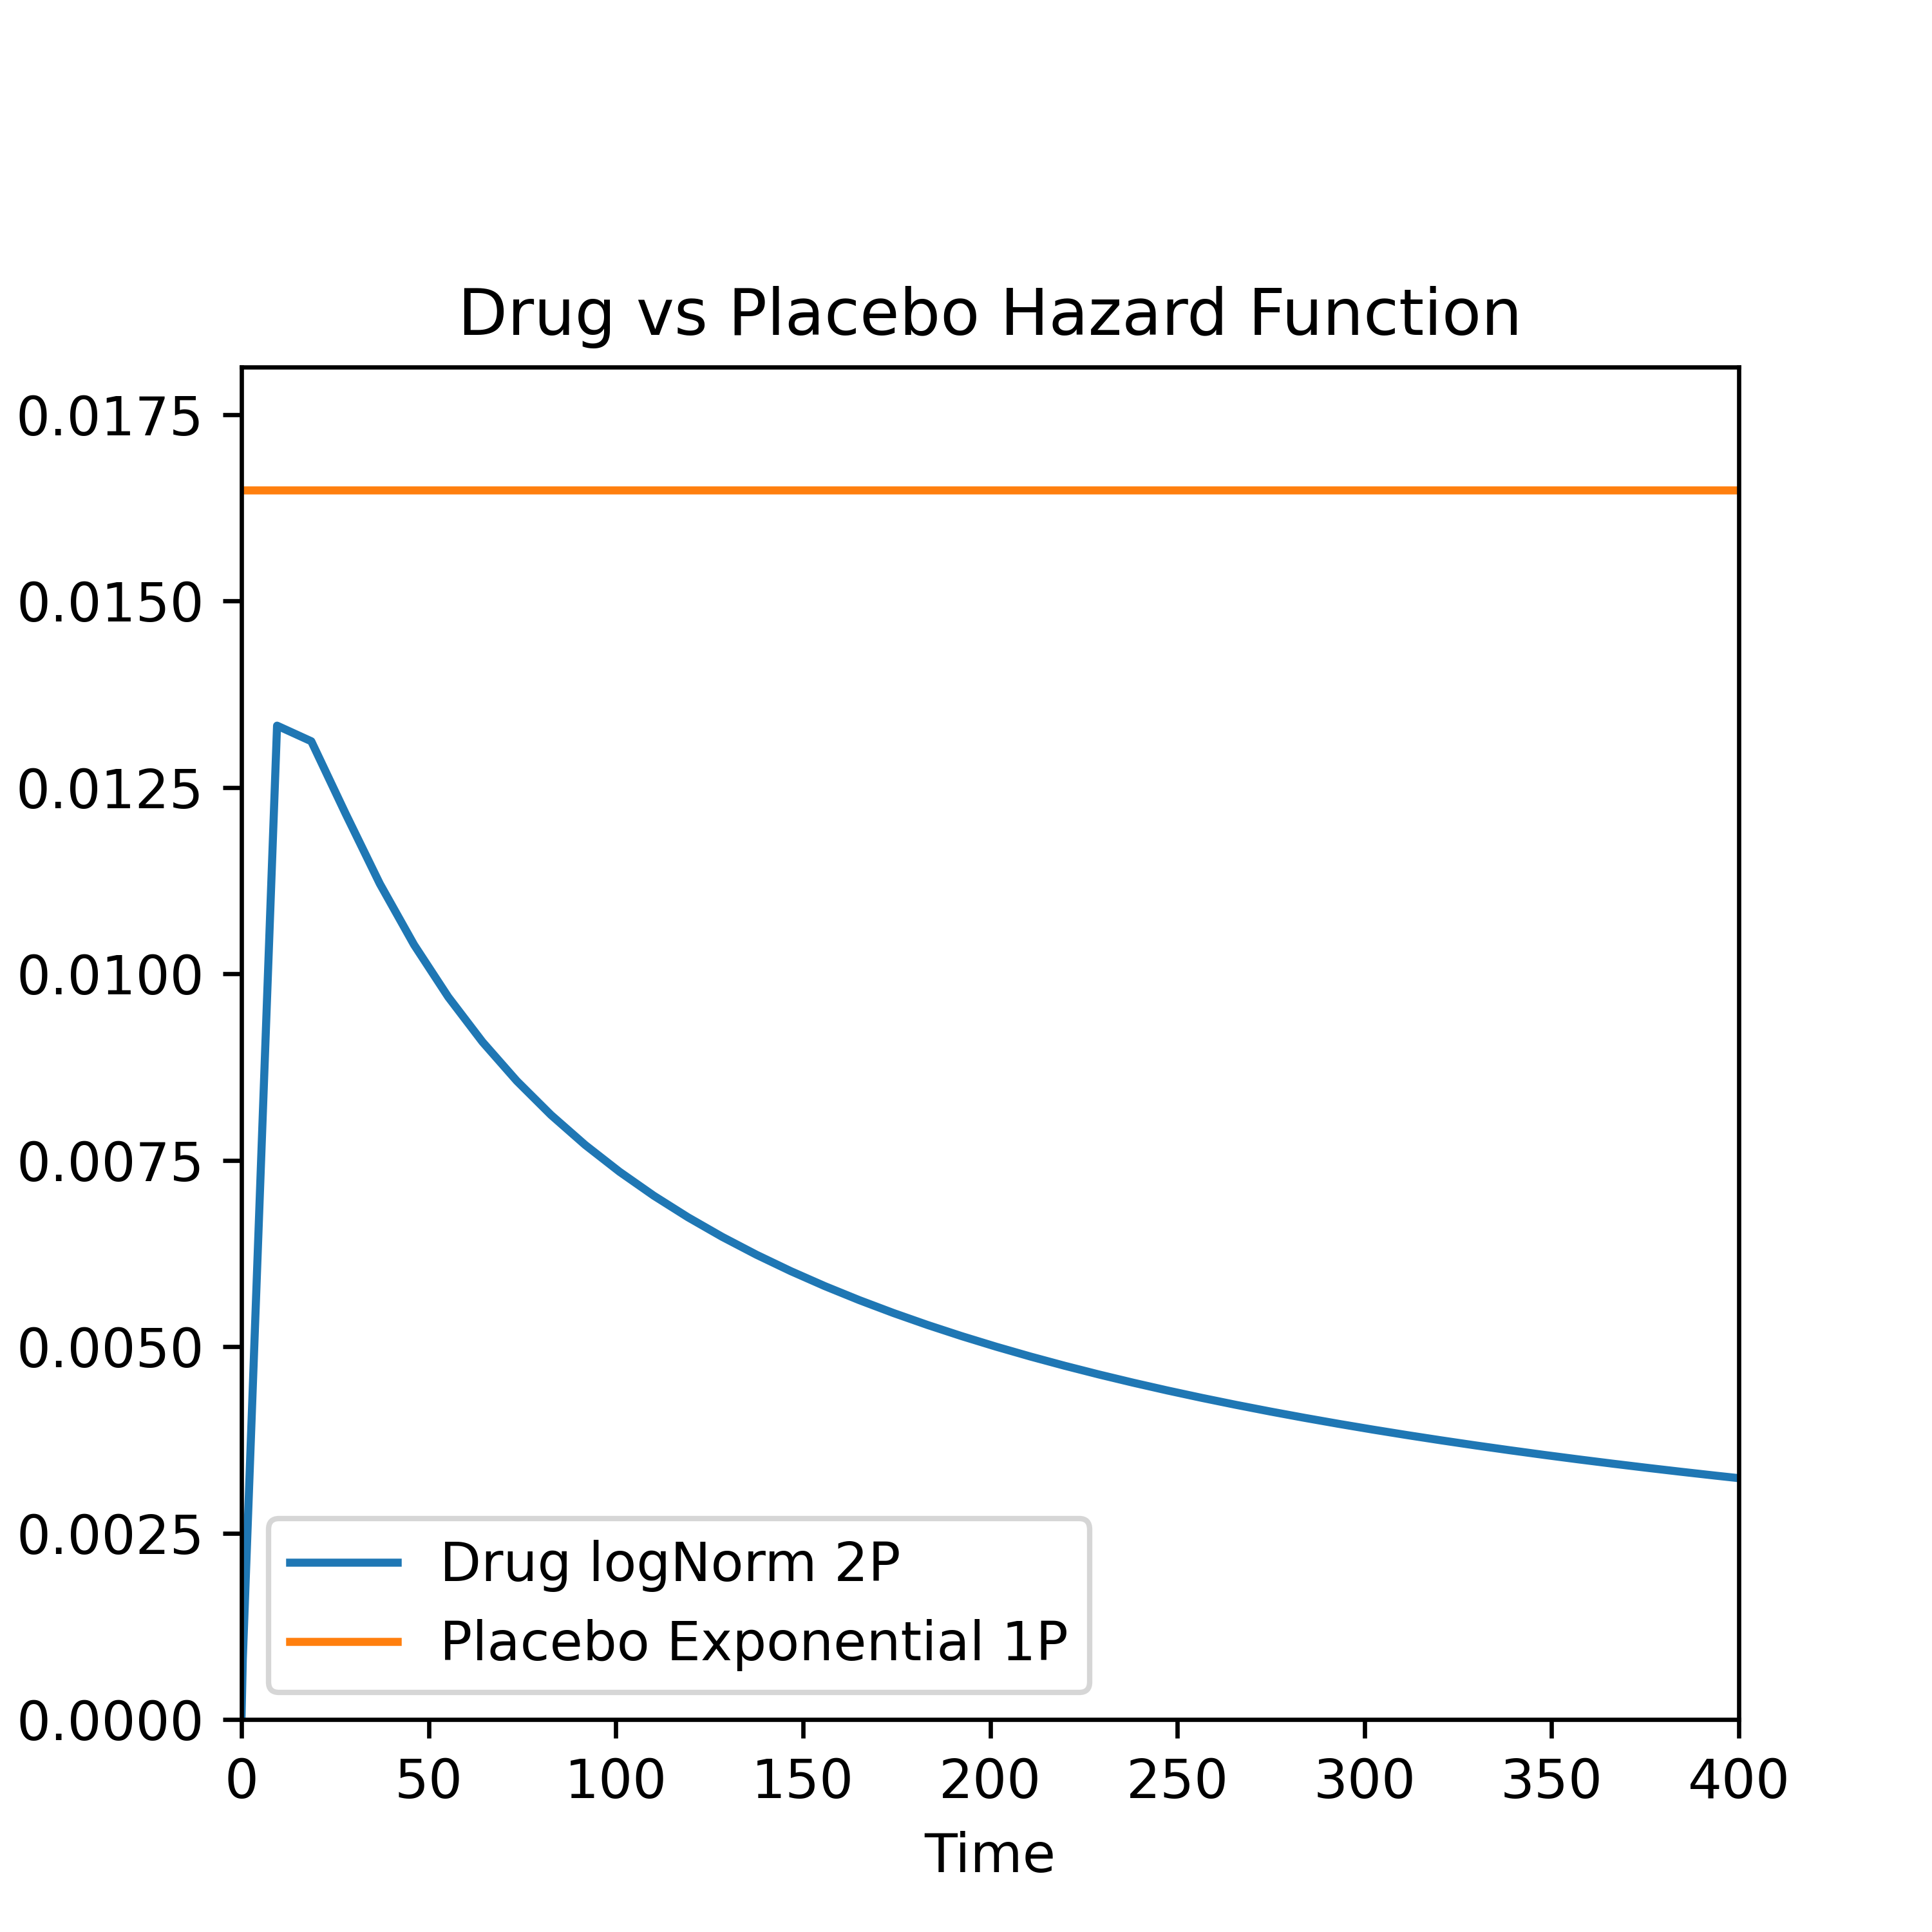
\includegraphics[width=0.5\linewidth]{img/hazard_rate_drug_vs_placebo_parametric_my_choice.png}
        \caption{Průběh intenzity poruch (\textit{hazard function}) pro vybrané parametrické modely}
        \label{fig:HF_for_parametric}
    \end{figure} 
    
   	\begin{figure}[H]
        \centering
        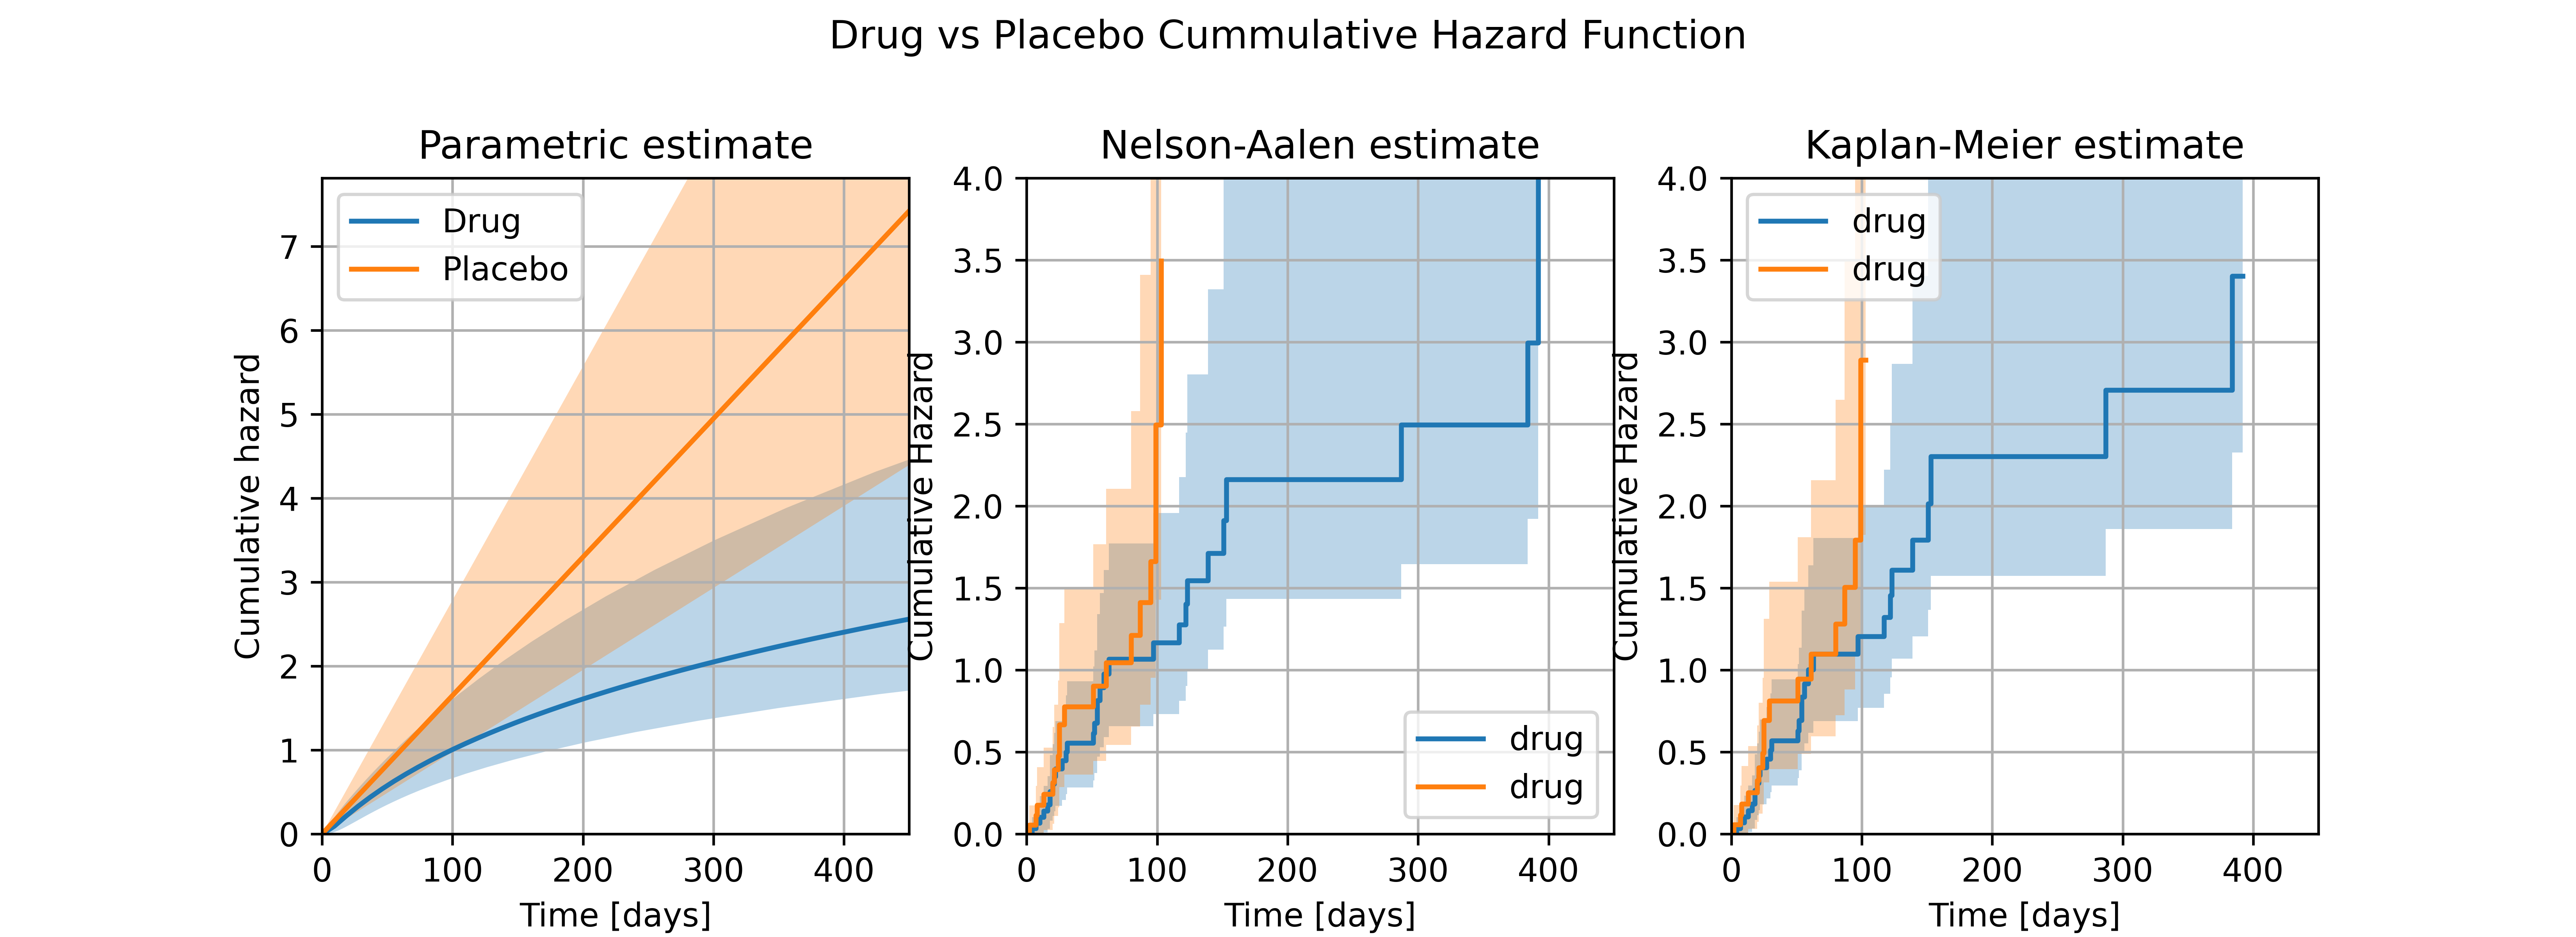
\includegraphics[width=1.0\linewidth]{img/cumulative_hazard_function_drug_vs_placebo_TRIPLE.png}
        \caption{Kumulativní intenzity poruch (\textit{cumulative hazard function})}
        \label{fig:CHF_for_parametric}
    \end{figure}     
    
    
    Vybrané číselné charakteristiky jsou uvedeny v tabulce níže.
 
\begin{table}[H]
    \centering
    \begin{tabular}{@{}lcrrr@{}}
        \toprule
        \multicolumn{1}{c}{Podskupina} & Použitý model & \multicolumn{1}{c}{MTTF {[}dnů{]}} & \multicolumn{1}{c}{$t_{\mbox{med}}$} & \multicolumn{1}{c}{MRL {[}dnů{]}} \\ \midrule
        \multirow{2}{*}{Lék}     & logNormal2P  & 163.64 & 62.11 & 270.4 \\
        & Kaplan-Meier & 129.95 & 54    &       \\
        \multirow{2}{*}{Placebo} & Exp1P        & 60.64  & 42.03 & 60.64 \\
        & Kaplan-Meier & 54.16  & 29    &       \\ \bottomrule
    \end{tabular}
    \caption{MRL = střední zbytková doba života (\textit{mean residual life}), MTTF = střední doba do úmrtí (\textit{mean time to failure}), $t_{\mbox{med}}$ = mediánová doba života}
    \label{tab:statistics}
\end{table}


%\begin{table}%[H]
%    \centering
%    \begin{tabular}{@{}|l|c|r|r|r|@{}}
%        \toprule
%        \multicolumn{1}{|c|}{Podskupina} & Použitý model & \multicolumn{1}{c|}{MTTF {[}dnů{]}} & \multicolumn{1}{c|}{$t_{\mbox{med}}$} & \multicolumn{1}{c|}{MRL {[}dnů{]}} \\ \midrule
%        \multirow{2}{*}{Lék}             &  logNormal2P  &                              163.64 &                                 62.11 &                              270.4 \\
%        \cmidrule(l){2-5}                & Kaplan-Meier  &                              129.95 &                                    54 &                                    \\ \midrule
%        \multirow{2}{*}{Placebo}         &     Exp1P     &                               60.64 &                                 42.03 &                              60.64 \\
%        \cmidrule(l){2-5}                & Kaplan-Meier  &                               54.16 &                                    29 &                                    \\ \bottomrule
%    \end{tabular}
%    \caption{MRL = střední zbytková doba života (mean resudual life), MTTF = střední doba do úmrtí (mean time to failure), $t_{\mbox{med}}$ = mediánová doba života}
%    \label{tab:statistics}
%\end{table}
    
    
	
	\newpage
	\section{Coxův regresní model} \label{sec:cox_model}
	\textit{Coxův regresní model} je založen na Coxově proporcionálním hazardovém předpokladu, který tvrdí, že poměrné riziko dvou skupin je konstantní v čase. Tento předpoklad umožňuje odhadnout vliv různých faktorů na přežití a současně zachovává nezávislost na neovlivňujících proměnných.
	
	Pro použití Coxova regresního modelu je nejprve potřeba mít k dispozici data o čase do události (např. úmrtí) a příslušné prediktory (faktory ovlivňující přežití). Zde byla použita existující implementace Coxova regresního modelu v knihovně \texttt{lifelines}.
	
	\subsection{Ověření předpokladů}
	Začněme vizuální kontrolou průběhů log-log $ \hat{R}_{KM} $ (Obrázek~\ref{fig:loglogplot_drug_vs_placebo}).
	 
	\begin{figure}[H]
		\centering
		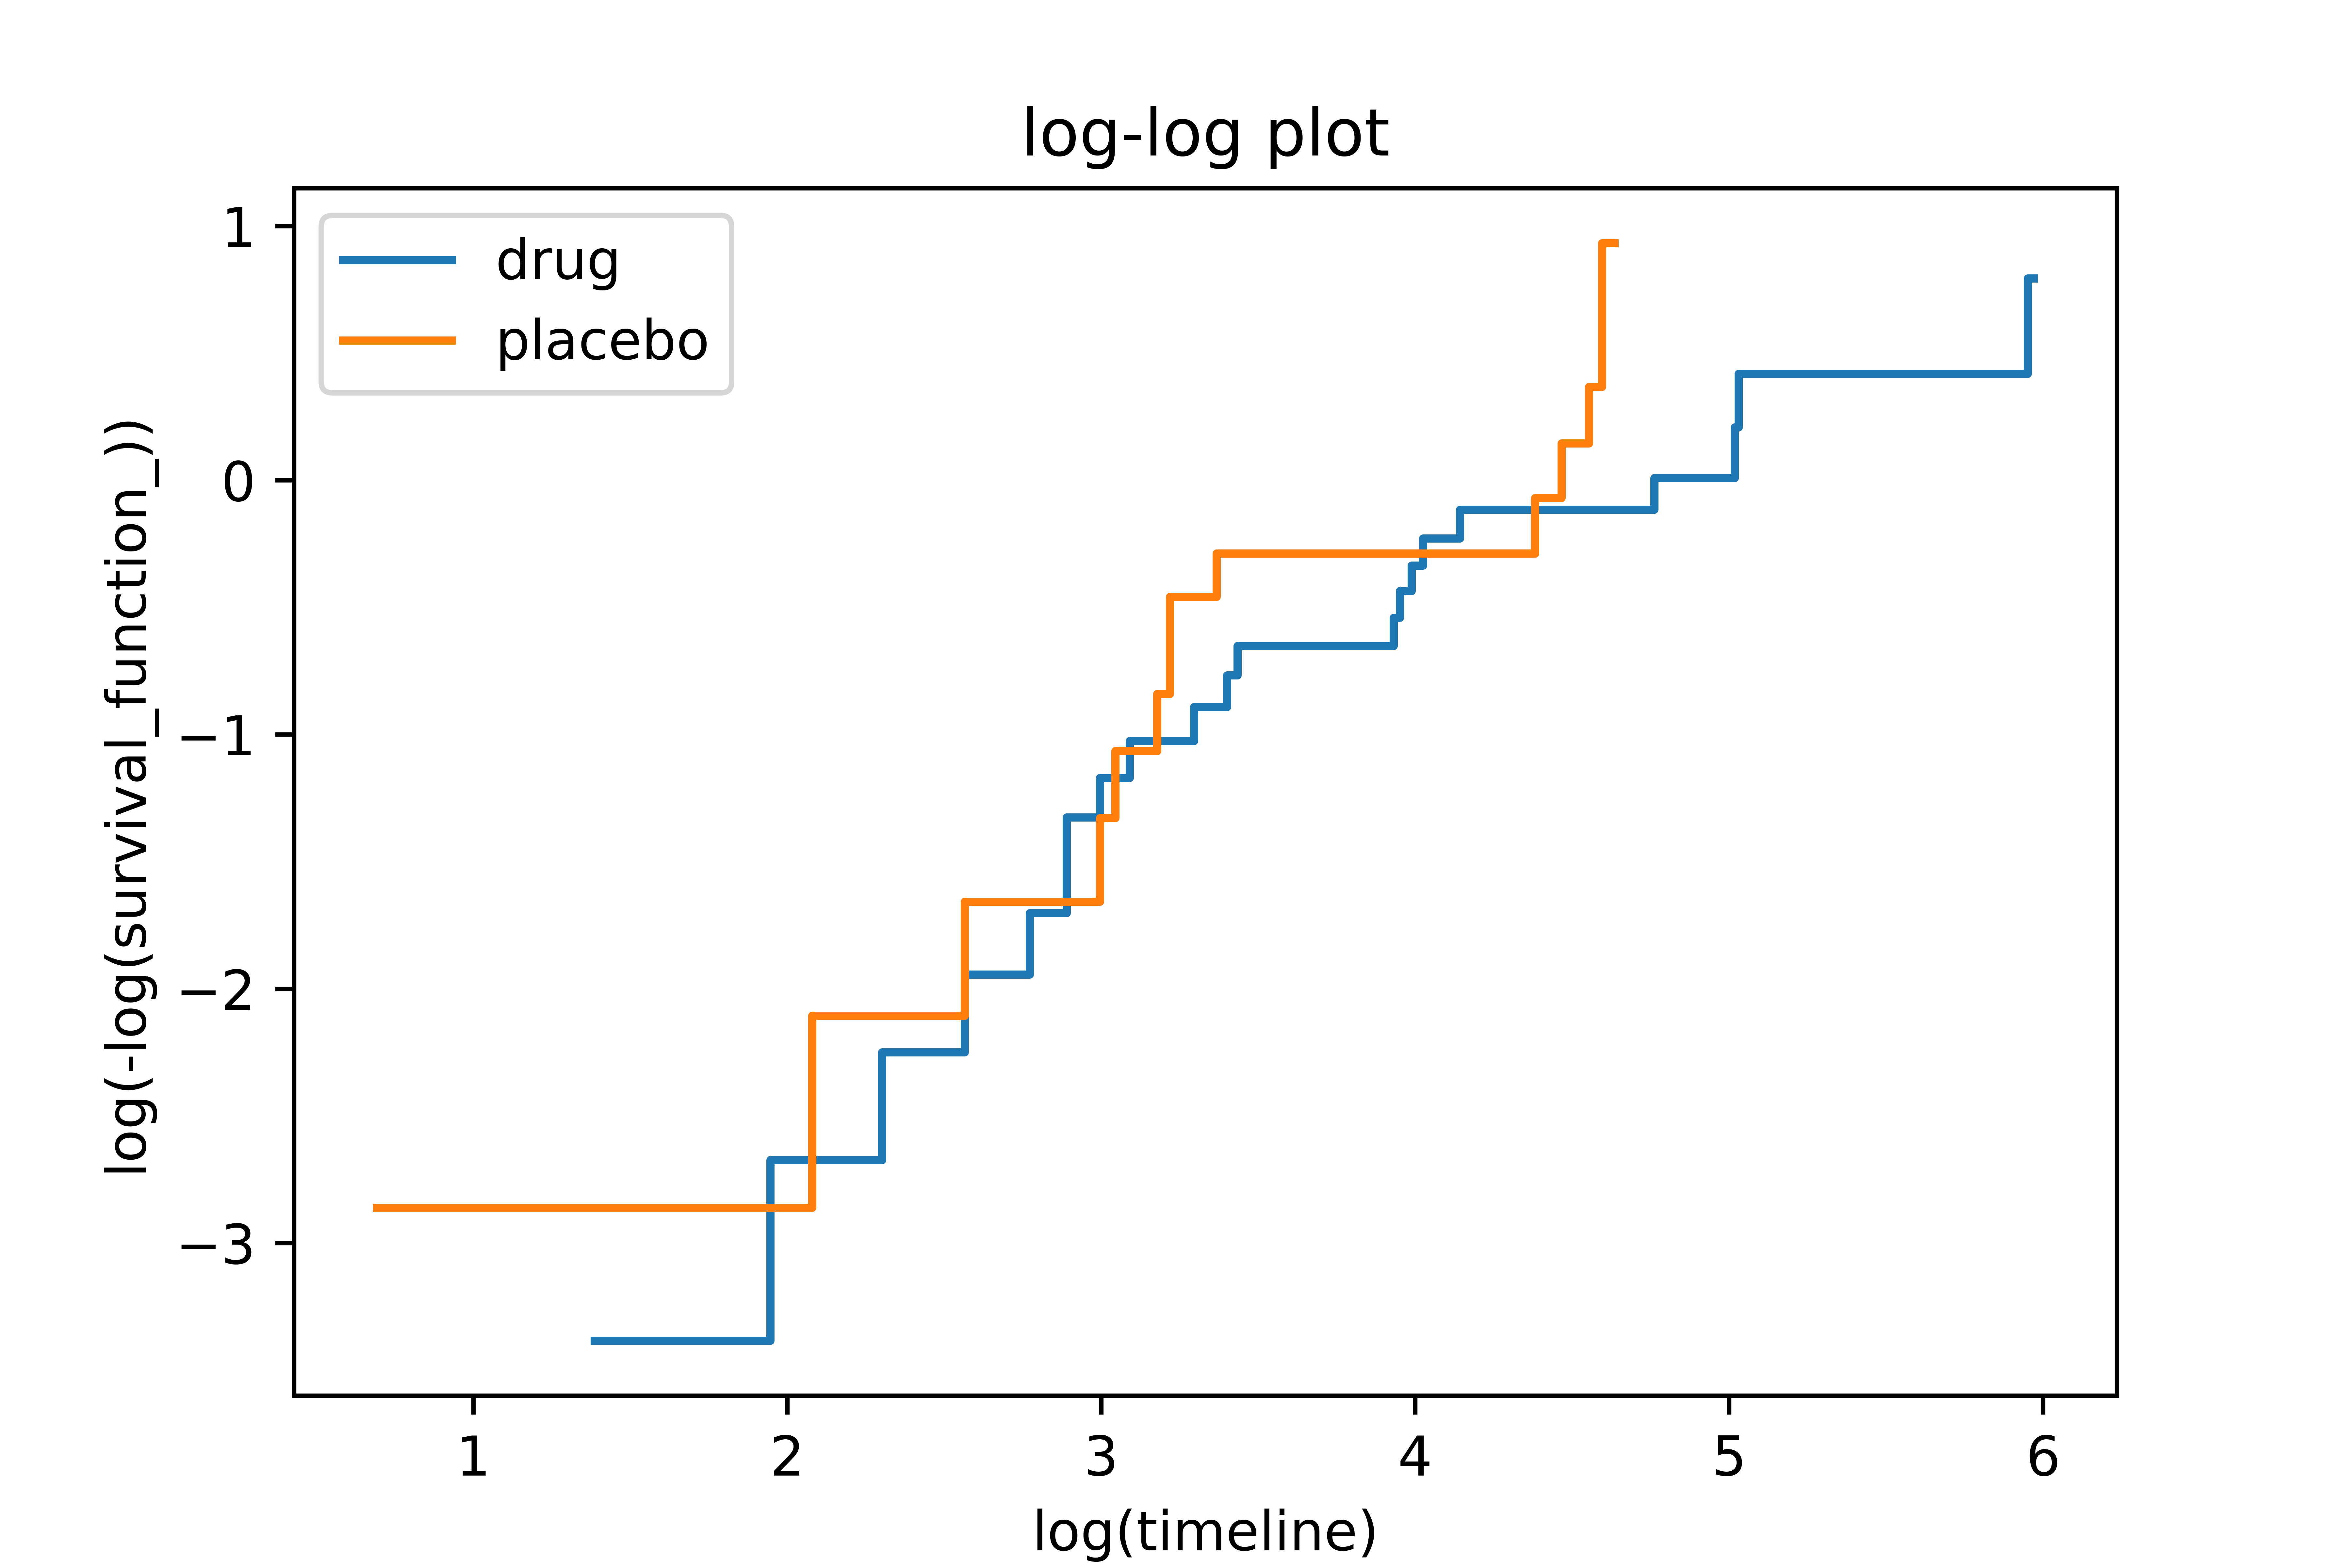
\includegraphics[width=0.6\linewidth]{img/loglogplot_KM.png}
	 	\caption{log-log plot lék vs placebo}
	 	\label{fig:loglogplot_drug_vs_placebo}
	\end{figure}
	
	Je vidět, že grafy nejsou \uvoz{rovnoběžné}, na několika místech se kříží. 
    Znamená to, že v tomto případě Coxův regresní model nelze použít. 

	%\subsection{Model}
    
    \begin{postulate}[DO NOT leave]
        Důvodem, proč nemohu použít Coxův proporcionální model rizik pro mou situaci, je přítomnost několika závažných problémů ve sbírce dat a vlastnostech mého datového souboru:
        
        1. Necenzurovaná data: Coxův model předpokládá, že data jsou cenzurována pouze zprava, což znamená, že neposkytuje adekvátní analýzu, pokud mám data cenzurována zleva nebo jsou nedostupná. Pokud je v mé datové sadě přítomnost těchto typů cenzury, mohou výsledky modelu být zkreslené a nepřesné.
        
        2. Nelinearita v efektech: Coxův model funguje nejlépe, pokud se předpokládá, že efekty proměnných jsou lineární v čase. Pokud mám důvody domnívat se, že efekty se mohou měnit nebo jsou nelineární, model nemusí poskytnout adekvátní odhady rizika.
        
        3. Interakce mezi proměnnými: Pokud existují interakce mezi proměnnými, které ovlivňují riziko, Coxův model může být problematický. Model nefunguje dobře při komplexních vztazích mezi proměnnými.
        
        4. Nízký počet událostí: Coxův model vyžaduje dostatečný počet událostí v porovnání s počtem proměnných, aby byl spolehlivý a stabilní. Pokud mám málo událostí ve srovnání s počtem proměnných, model může vykazovat nedostatečnou přesnost.
        
        5. Nezávislé pozorování: Coxův model předpokládá, že pozorování jsou nezávislá. Pokud mám v datech přítomnost korelovaných nebo shlukovaných pozorování, může to model zpochybnit.
        
        Vzhledem k těmto omezením je vhodné hledat alternativní modely, které lépe odpovídají charakteru mých dat a umožní spolehlivě odhadnout riziko ve zkoumaném kontextu.
    \end{postulate}
    
	
	\newpage
	\section{Závěr}\label{sec:zaver}
	Tato práce 

\end{document}